
\documentclass{beamer}	
\mode<presentation>
 
\usepackage{pdfpages}
\usepackage{fancyvrb}
\usepackage{chemarr}

\usepackage{amsmath}		%% mathematics typesetting
\usepackage{amssymb}
 
\usepackage{ulem}

\usepackage{booktabs}

\usepackage{siunitx} %% tpyeset SI units

\usepackage{CJKutf8} %% typeset Chinese characters

\usepackage{pdfpages}

% Color and Theme. Can be changed. However, this one's quite nice.
\usetheme{Madrid}
\definecolor{theme}{rgb}{0.84,0,0.21}
\usecolortheme[named=theme]{structure}


%%  Title information
\title[M01.1 Grundbegriffe]{M01.1 Grundbegriffe, Methodik, Fehlerrechnung}
\author[melanie.stefan@medicalschool-berlin.de]{M01 Physik für Mediziner*innen}
\institute[]{Prof. Melanie Stefan - melanie.stefan@medicalschool-berlin.de}
\date{SoSe 2023}
 

% Table of contents to pop up at the beginning of each section
\AtBeginSection[]
{
  \begin{frame}<beamer>
    \frametitle{Outline}
    \tableofcontents[currentsection,currentsubsection]
  \end{frame}
}
 
\beamertemplatenavigationsymbolsempty

\begin{document}
 
 
 
{ \usebackgroundtemplate{
\includegraphics[width=1.2\paperwidth]{MSB_Titelseite.pdf}} 
\begin{frame}

 \maketitle 

$\,$\\[6cm] 


\end{frame} 
}


\begin{frame}
\frametitle{Herzlich Willkommen an der MSB}




\end{frame}

\begin{frame}
\frametitle{Was kommt auf Sie zu?}

\begin{center}
    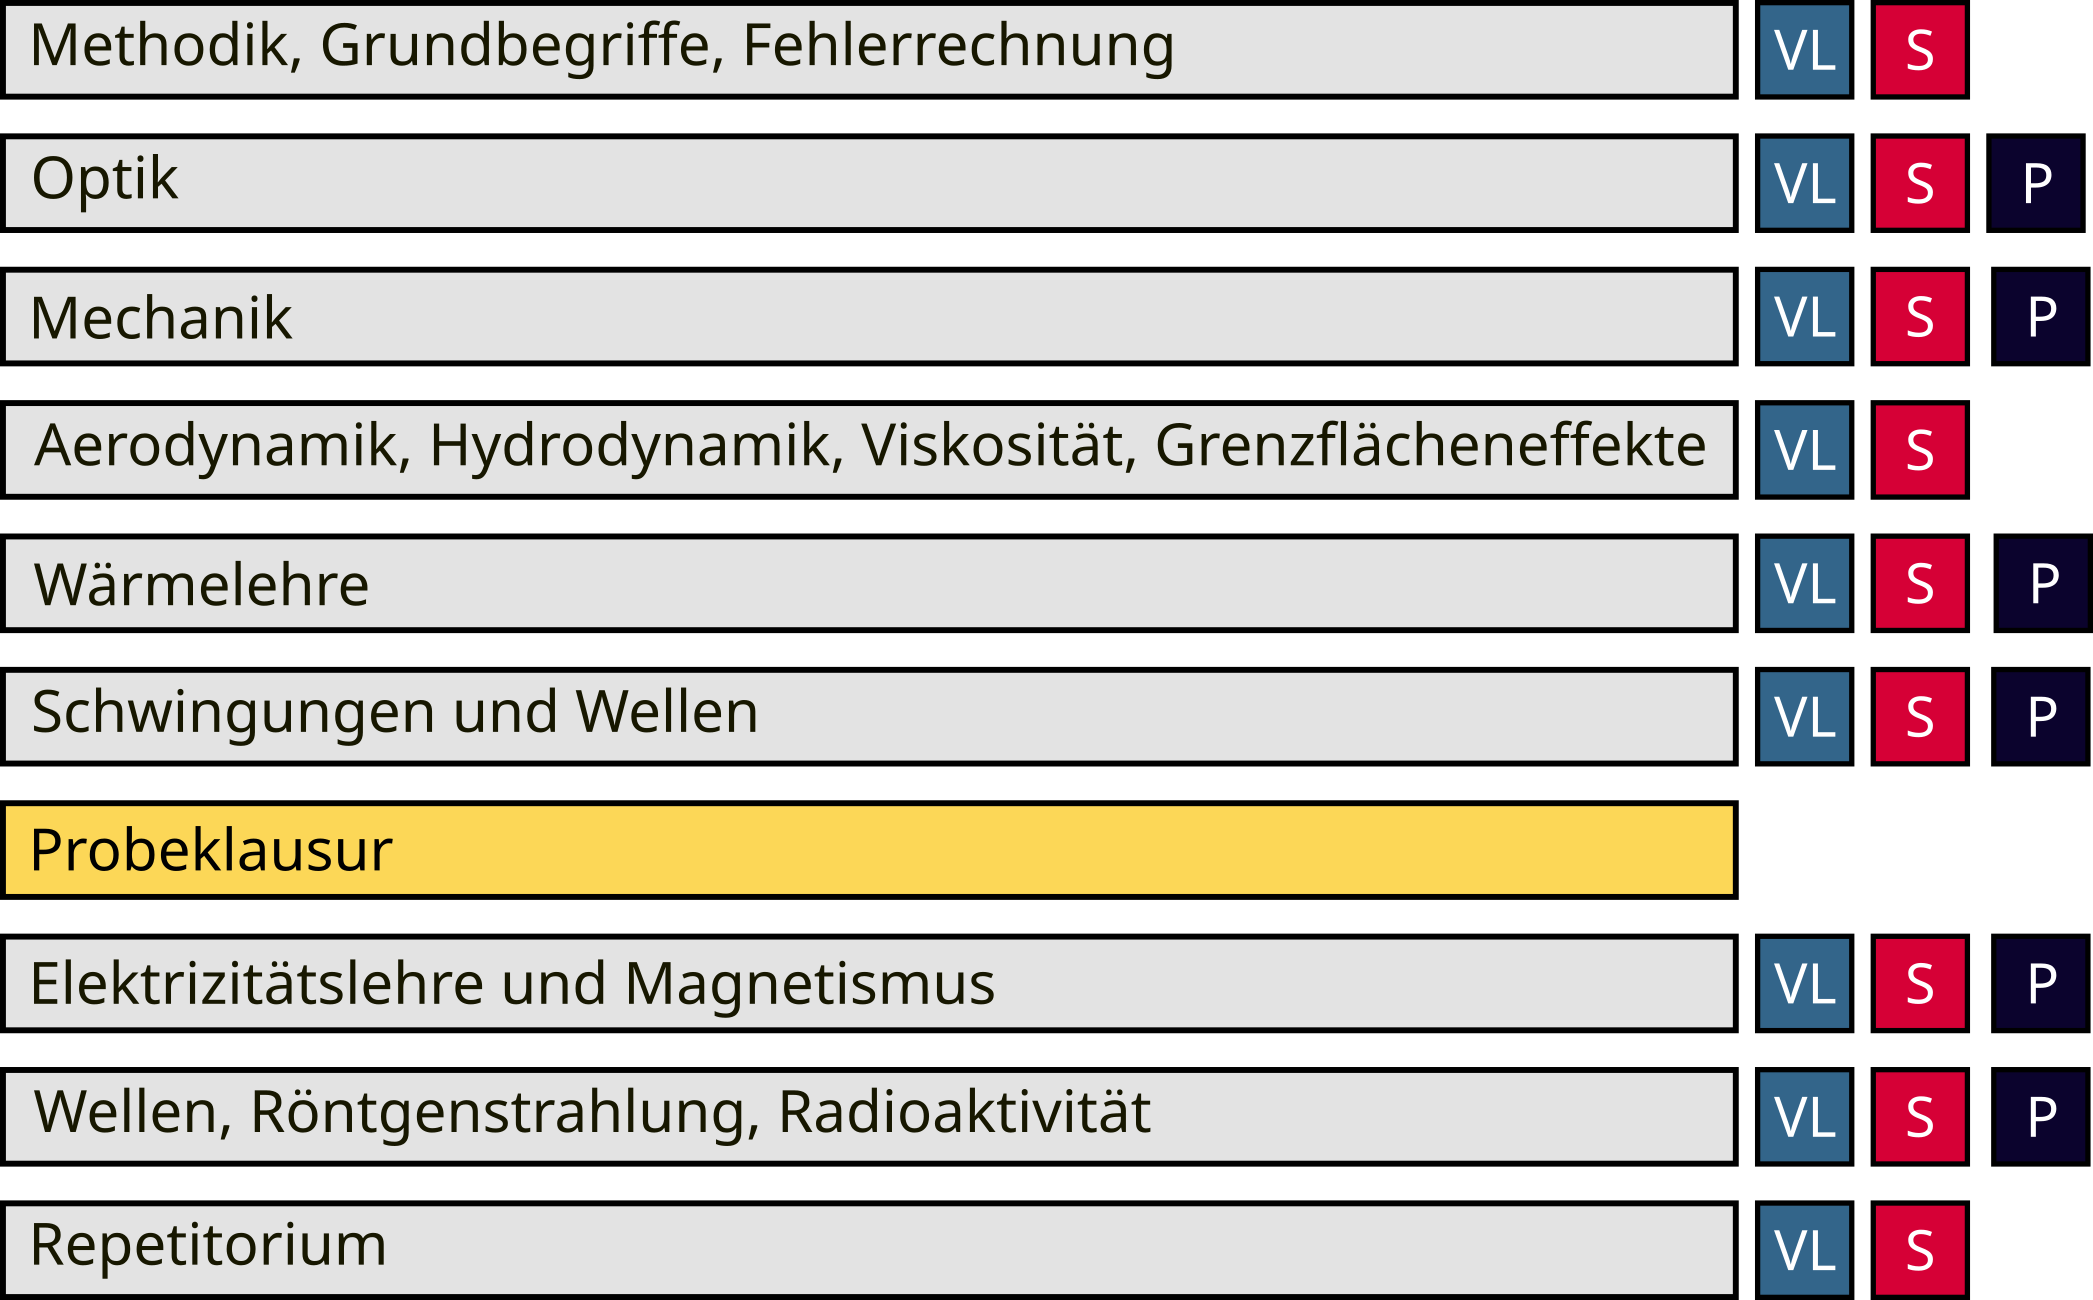
\includegraphics[width=\textwidth]{physik_module.png}
\end{center}

\end{frame}
 

%% Hook
\begin{frame}
\frametitle{Neulich in der Zeitung \dots}

\begin{center}
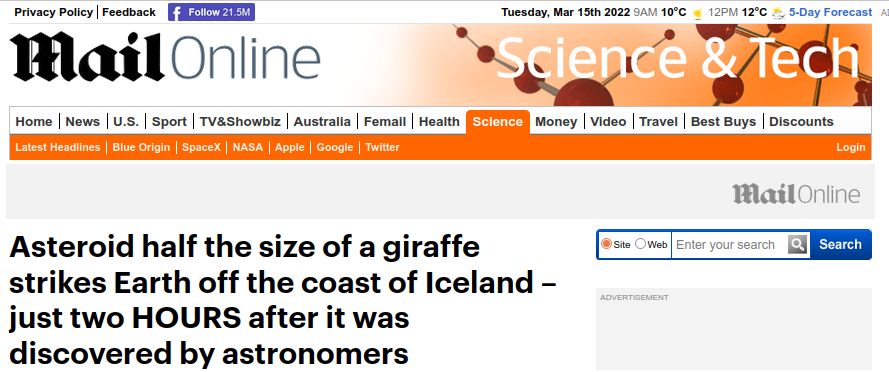
\includegraphics[width=\textwidth]{giraffe.png}
\end{center}

 
\end{frame}

%% TLIA
\begin{frame}
\frametitle{In dieser Vorlesung geht es um \dots}

\dots das \textcolor{theme}{Messen} und \textcolor{theme}{Darstellen} von und \textcolor{theme}{Rechnen} mit Daten.

\begin{center}
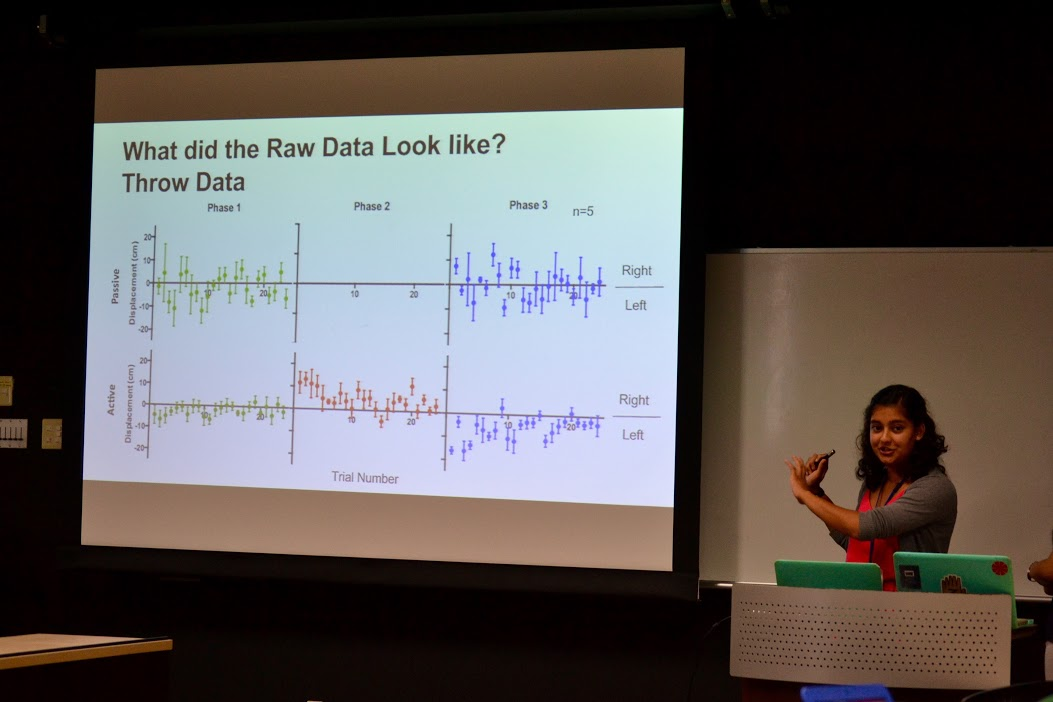
\includegraphics[width=\textwidth]{student_presenting.jpg}

\end{center}

 
\end{frame}



%% Learning Objectives

\begin{frame}

\frametitle{Nach dieser Vorlesung sollten Sie:}



\begin{block}{Wissen:}
\begin{itemize}
\item
Basiseinheiten und häufige abgeleitete Einheiten des SI-Systems benennen
\item
Messunsicherheit erklären
\item
 Vektoren, Skalare, Exponentialfunktionen, Logarithmen, Trigonometrischen Funktionen, Integration und Differentialrechnung erklären
\item 
Mittelwert, Standardabweichung, und Standardabweichung des Mittelwerts erklären 
\item
Eigenschaften der Gaußschen Glockenkurve benennen
\end{itemize}
\end{block}

\end{frame}

\begin{frame}

\frametitle{Nach dieser Vorlesung sollten Sie:}
 



\begin{block}{Können:}
\begin{itemize}
\item
 dezimale Vielfache von Einheiten sprachlich und durch Zehnerpotenzen darstellen
\item
 mit Messgrößen rechnen
\item
 Messunsicherheit darstellen und abschätzen
\item
 Mittelwert, Standardabweichung, und Standardabweichung des Mittelwerts berechnen
\item 
mit Funktionsgraphen arbeiten
\end{itemize}
\end{block}

\pause
 
\begin{block}{Fühlen:}
\begin{itemize}
\item
erkennen, warum Physik in der Medizin wichtig ist
\item
verstehen, warum manche Konzepte (Gaußsche Glockenkurve, Logarithmen, Differential etc.) oft vorkommen
\item
 rechnen ohne Angst
\end{itemize}
\end{block}

\end{frame}

%% Main Body

\section{Messen}


%% Giraffe: Was ist messen?
\begin{frame}
\frametitle{Was ist Messen}

\textbf{Messen} ist der Vergleich einer Messgröße mit ihrer Einheit

\[
\text{Maßzahl} = \text{Zahl} \times \text{Einheit}
\]


\begin{center}
\includegraphics<1>[width=0.8\textwidth]{messen_no_anno.png}
\includegraphics<2>[width=0.8\textwidth]{messen.png}
\end{center}

Was ist das Problem mit der Maßeinheit ``Giraffe''?

 
\end{frame}


\begin{frame}
\frametitle{Was ist das Problem mit der Maßeinheit ``Giraffe''?}


\begin{columns}

\begin{column}{5cm}


\begin{itemize}
\item
Was für eine Giraffe? (Alt? Jung?)  
\item
Welche Eigenschaft der Giraffe wird überhaupt verwendet? (Höhe? Gewicht? Volumen?)

\end{itemize}

\end{column}

\begin{column}{5cm}

\begin{center}
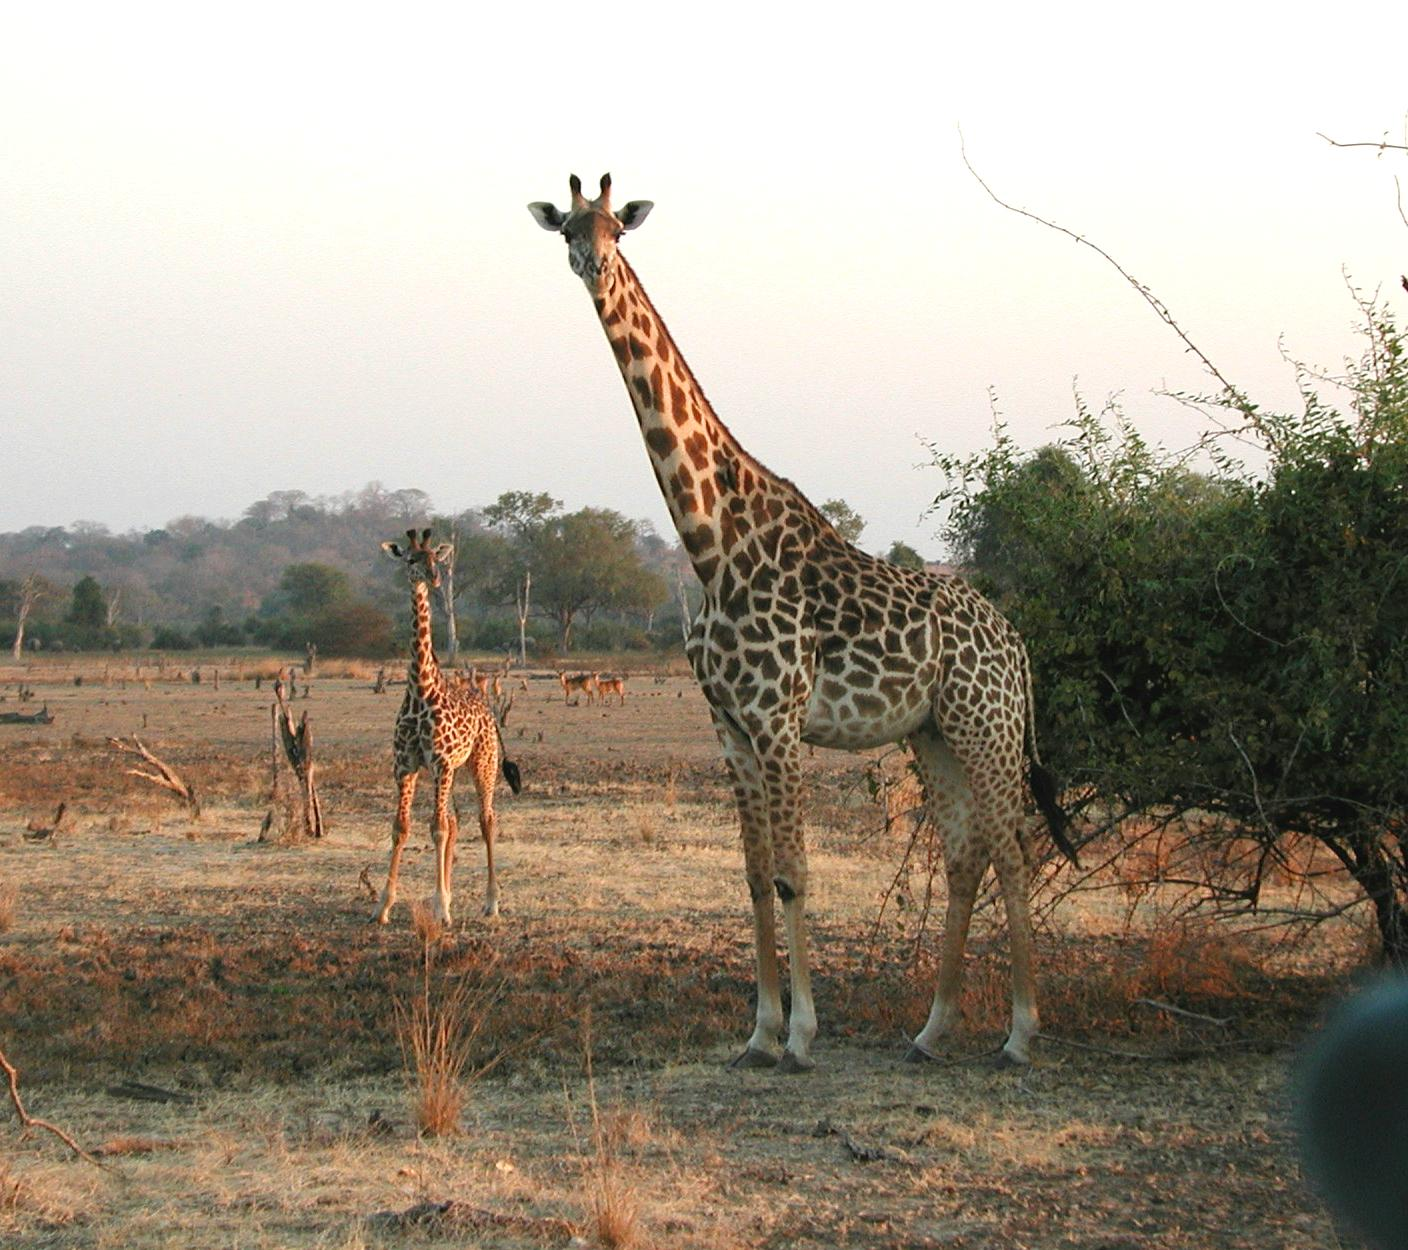
\includegraphics[width=\textwidth]{Giraffen.jpg}
\end{center}



\end{column}
 


\end{columns}


$\,$\\[0.5 cm]
Wir brauchen Maßeinheiten, auf die wir uns einigen können! 

\end{frame}


%% SI Einheiten 

\begin{frame}

\frametitle{Das Internationale Einheitensystem (SI)}


\begin{block}{Grundgrößen}
1. die Länge mit der Einheit Meter (m) \\
2. die Zeit mit der Einheit Sekunde (s) \\
3. die Masse mit der Einheit Kilogramm (kg) \\
4. die elektrische Stromstärke mit der Einheit Ampère (A) \\
5. die Temperatur mit der Einheit Kelvin (K) \\
6. die Stoffmenge mit der Einheit Mol (mol) \\
7. die Lichtstärke mit der Einheit Candela (cd) \\
\end{block}

\pause

Alle anderen Einheiten werden aus den Grundeinheiten zusammengesetzt. 

\end{frame}


\begin{frame}
\frametitle{Umrechnen von Einheiten}
%% Umrechnen: Giraffe to m?

\[1\, \text{Giraffe} \sim 6\,\text{m} \]

\[
1\,\text{Asteroid} = 0,5\, \text{Giraffe} \times 6\, \frac{\text{m}}{\text{Giraffe}} = 3\,\text{m}
\]


\end{frame}

%% Umrechnen (Übung) Giraffe to kg

\begin{frame}
\frametitle{Kleine schnelle Übung}
%% Umrechnen: Giraffe to kg?

\[1\, \text{Giraffe} \sim 1600\,\text{kg} \]

\[
1\,\text{Asteroid} =  ?
\]


\end{frame}


\begin{frame}
\frametitle{Umrechnen von Einheiten}
%% Umrechnen: Giraffe to m?

\[1\, \text{Giraffe} \sim 1600\,\text{kg} \]

\[
1\,\text{Asteroid} =  0,5\, \text{Giraffe} \times 1600\, \frac{\text{kg}}{\text{Giraffe}} = 800\,\text{kg}
\]


\end{frame}



%% Vielfache von Einheiten

\begin{frame}
\frametitle{Weiter Messbereich in der Medizin}
\begin{tabular}{ll}
Giraffe & \SI{6}{m} \\
\\
\\
\\
\\
\\
\\
\end{tabular}
\end{frame}

\begin{frame}
\frametitle{Weiter Messbereich in der Medizin}
\begin{tabular}{ll}
\sout{Giraffe} & \sout{6\,m} \\
\\
\\
\\
\\
\\
\\
\end{tabular}
\end{frame}
 
\begin{frame}
\frametitle{Weiter Messbereich in der Medizin}
\begin{tabular}{ll}
Mensch & \SI{1,7}{m} \\
\pause
Länge eines Auges       & \SI{0,024}{m} \\
Dicke eines Haares      & \SI{0,000 1 }{m} \\
Dicke von E. coli       & \SI{0,000 001}{m} \\
Protein                 & \SI{0,000 000 005}{m} \\
Wasserstoffatom         & \SI{0,000 000 000 1}{m} \\ 
Proton                  & \SI{0,000 000 000 000 001 7}{m} \\
\end{tabular}
\end{frame}

\begin{frame}
\frametitle{Angaben in Zehnerpotenzen}
\begin{tabular}{lll}
Mensch                  & \SI{1,7}{m}   & \SI{1,7e0}{m} \\
Länge eines Auges       & \SI{0,024}{m} & \SI{24e-3}{m}  \\
Dicke eines Haares      & \SI{0,000 1 }{m} & ? \\
Dicke von E. coli       & \SI{0,000 001}{m} \\
Protein                 & \SI{0,000 000 005}{m} \\
Wasserstoffatom         & \SI{0,000 000 000 1}{m} \\ 
Proton                  & \SI{0,000 000 000 000 001 7}{m} \\
\end{tabular}
\end{frame} 



\begin{frame}
\frametitle{Angaben in Zehnerpotenzen}
\begin{tabular}{llll}
Mensch                  & \SI{1,7}{m}   & \SI{1,7e0}{m} \\
Länge eines Auges       & \SI{0,024}{m} & \SI{24e-3}{m}  \\
Dicke eines Haares      & \SI{0,000 1 }{m} &  \SI{1e-4}{m}  \\
Dicke von E. coli       & \SI{0,000 001}{m} & \SI{1e-6}{m}  \\
Protein                 & \SI{0,000 000 005}{m} & \SI{5e-9}{m}\\
Wasserstoffatom         & \SI{0,000 000 000 1}{m} & \SI{1e-10}{m} \\ 
Proton                  & \SI{0,000 000 000 000 001 7}{m}& \SI{1,7e-15}{m} \\
\end{tabular}
\end{frame} 


\begin{frame}
\frametitle{(Noch bessere) Angaben in Zehnerpotenzen}
\begin{tabular}{llll}
Mensch                  & \SI{1,7}{m}   & \SI{1,7e0}{m} \\
Länge eines Auges       & \SI{0,024}{m} & \SI{24e-3}{m}  \\
Dicke eines Haares      & \SI{0,000 1 }{m} &  \textcolor{theme}{\SI{0,1e-3}{m}}  \\
Dicke von E. coli       & \SI{0,000 001}{m} & \SI{1e-6}{m}  \\
Protein                 & \SI{0,000 000 005}{m} & \SI{5e-9}{m}\\
Wasserstoffatom         & \SI{0,000 000 000 1}{m} & \textcolor{theme}{\SI{100e-12}{m}} \\ 
Proton                  & \SI{0,000 000 000 000 001 7}{m}& \SI{1,7e-15}{m} \\
\end{tabular}
\end{frame} 

\begin{frame}
\makebox[\linewidth]{
\includegraphics[page=20,width=\textwidth]{Walter.pdf}}
\end{frame}


\begin{frame}
\frametitle{(Noch bessere) Angaben in Zehnerpotenzen}
\begin{tabular}{llll}
Mensch                  & \SI{1,7}{m}   & \SI{1,7}{m} \\
Länge eines Auges       & \SI{0,024}{m} & \SI{24}{\milli\meter}  \\
Dicke eines Haares      & \SI{0,000 1 }{m} &  \SI{0,1}{\milli\meter}  \\
Dicke von E. coli       & \SI{0,000 001}{m} & \SI{1}{\micro\meter}  \\
Protein                 & \SI{0,000 000 005}{m} & \SI{5}{\nano\meter}\\
Wasserstoffatom         & \SI{0,000 000 000 1}{m} & \SI{100}{\pico \meter} \\ 
Proton                  & \SI{0,000 000 000 000 001 7}{m}& \SI{1,7}{\femto\meter} \\
\end{tabular}
\end{frame} 


\begin{frame}
\makebox[\linewidth]{
\includegraphics[page=15,width=\textwidth]{Walter.pdf}}
\end{frame}


%% Giraffe Volumen? 
\begin{frame}
\frametitle{Was, wenn das Volumen der Giraffe gemeint war?}

\begin{center}
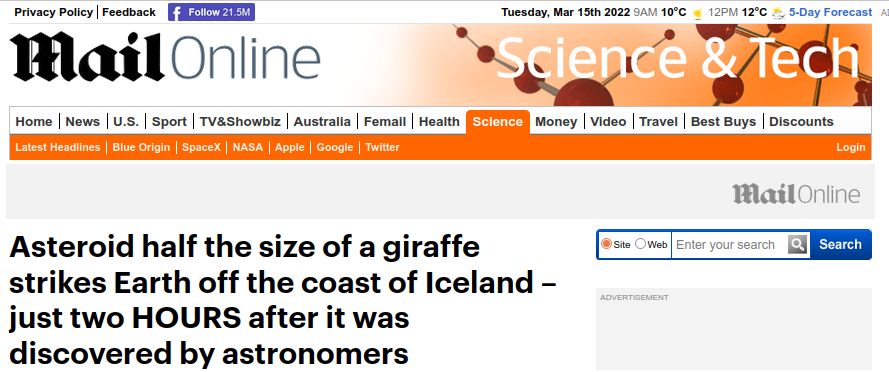
\includegraphics[width=\textwidth]{giraffe.png}
\end{center}

\end{frame}



% \begin{frame}{Zusammengesetzte Einheiten}

% \begin{block}{Aus einer SI-Einheit - Beispiele}
% \begin{itemize}
%     \item 
% Fläche (A) in m$^2$
% \item
% Volumen (V) in m$^3$
% \item
% Frequenz (f) in s$^{-1}$ (Auch: Hertz, $1\,\text{Hz} =  1\,\text{s}^{-1}$
% \end{itemize}
    
% \end{block}


% \begin{block}{Aus mehreren SI-Einheiten - Beispiele}
% \begin{itemize}
%     \item 
% \end{itemize}
    
% \end{block}


% \end{frame}



\begin{frame}
\frametitle{Was ist das Volumen einer Giraffe?}

 
\begin{center}
\includegraphics<1>[width=0.6\textwidth]{giraffe_volumen_1.png}
\includegraphics<2>[width=0.6\textwidth]{giraffe_volumen_2.png}
\end{center}



\end{frame}


\begin{frame}
\frametitle{Was ist das Volumen einer Giraffe?}


\[ 
\text{Dichte}  = \frac{\text{Masse}}{\text{Volumen}}
\]

\[
\text{Volumen} =  \frac{\text{Masse}}{\text{Dichte}} 
\]


\end{frame}

\begin{frame}
\frametitle{Was ist das Volumen einer Giraffe?}


\[ 
\text{Dichte}  = \frac{\text{Masse}}{\text{Volumen}}
\]
 
\[
\text{Volumen} =  \frac{1600\,\text{kg}}{\text{Dichte}} 
\]



\end{frame}


\begin{frame}
\frametitle{Was ist das Volumen einer Giraffe?}


\[ 
\text{Dichte}  = \frac{\text{Masse}}{\text{Volumen}}
\]
 
\[
\text{Volumen} =  \frac{1600\,\text{kg}}{1000\,\frac{\text{kg}}{\text{m}^3}} 
\]


\pause

(Giraffen sind hauptsächlich aus Wasser)


\end{frame}


\begin{frame}
\frametitle{Was ist das Volumen einer Giraffe?}


\[ 
\text{Dichte}  = \frac{\text{Masse}}{\text{Volumen}}
\]
 
\[
\text{Volumen} =  \frac{1600\,\text{kg}}{1000\,\frac{\text{kg}}{\text{m}^3}} =    1.6\,\text{m}^3
\]


\end{frame}

 

\begin{frame}
\makebox[\linewidth]{
\includegraphics[page=44,width=\textwidth]{Walter.pdf}}
\end{frame}


\section{Darstellen}

%% Mittelwert, Standardabweichung, SEM
\begin{frame}
\frametitle{Wie können wir gemessene Daten darstellen?}

Beispiel: Körpergewicht (in kg) und Dauer eines 5-Kilometer-Laufs (in s) von 14 zufällig ausgewählten Erwachsenen
 
\begin{center}
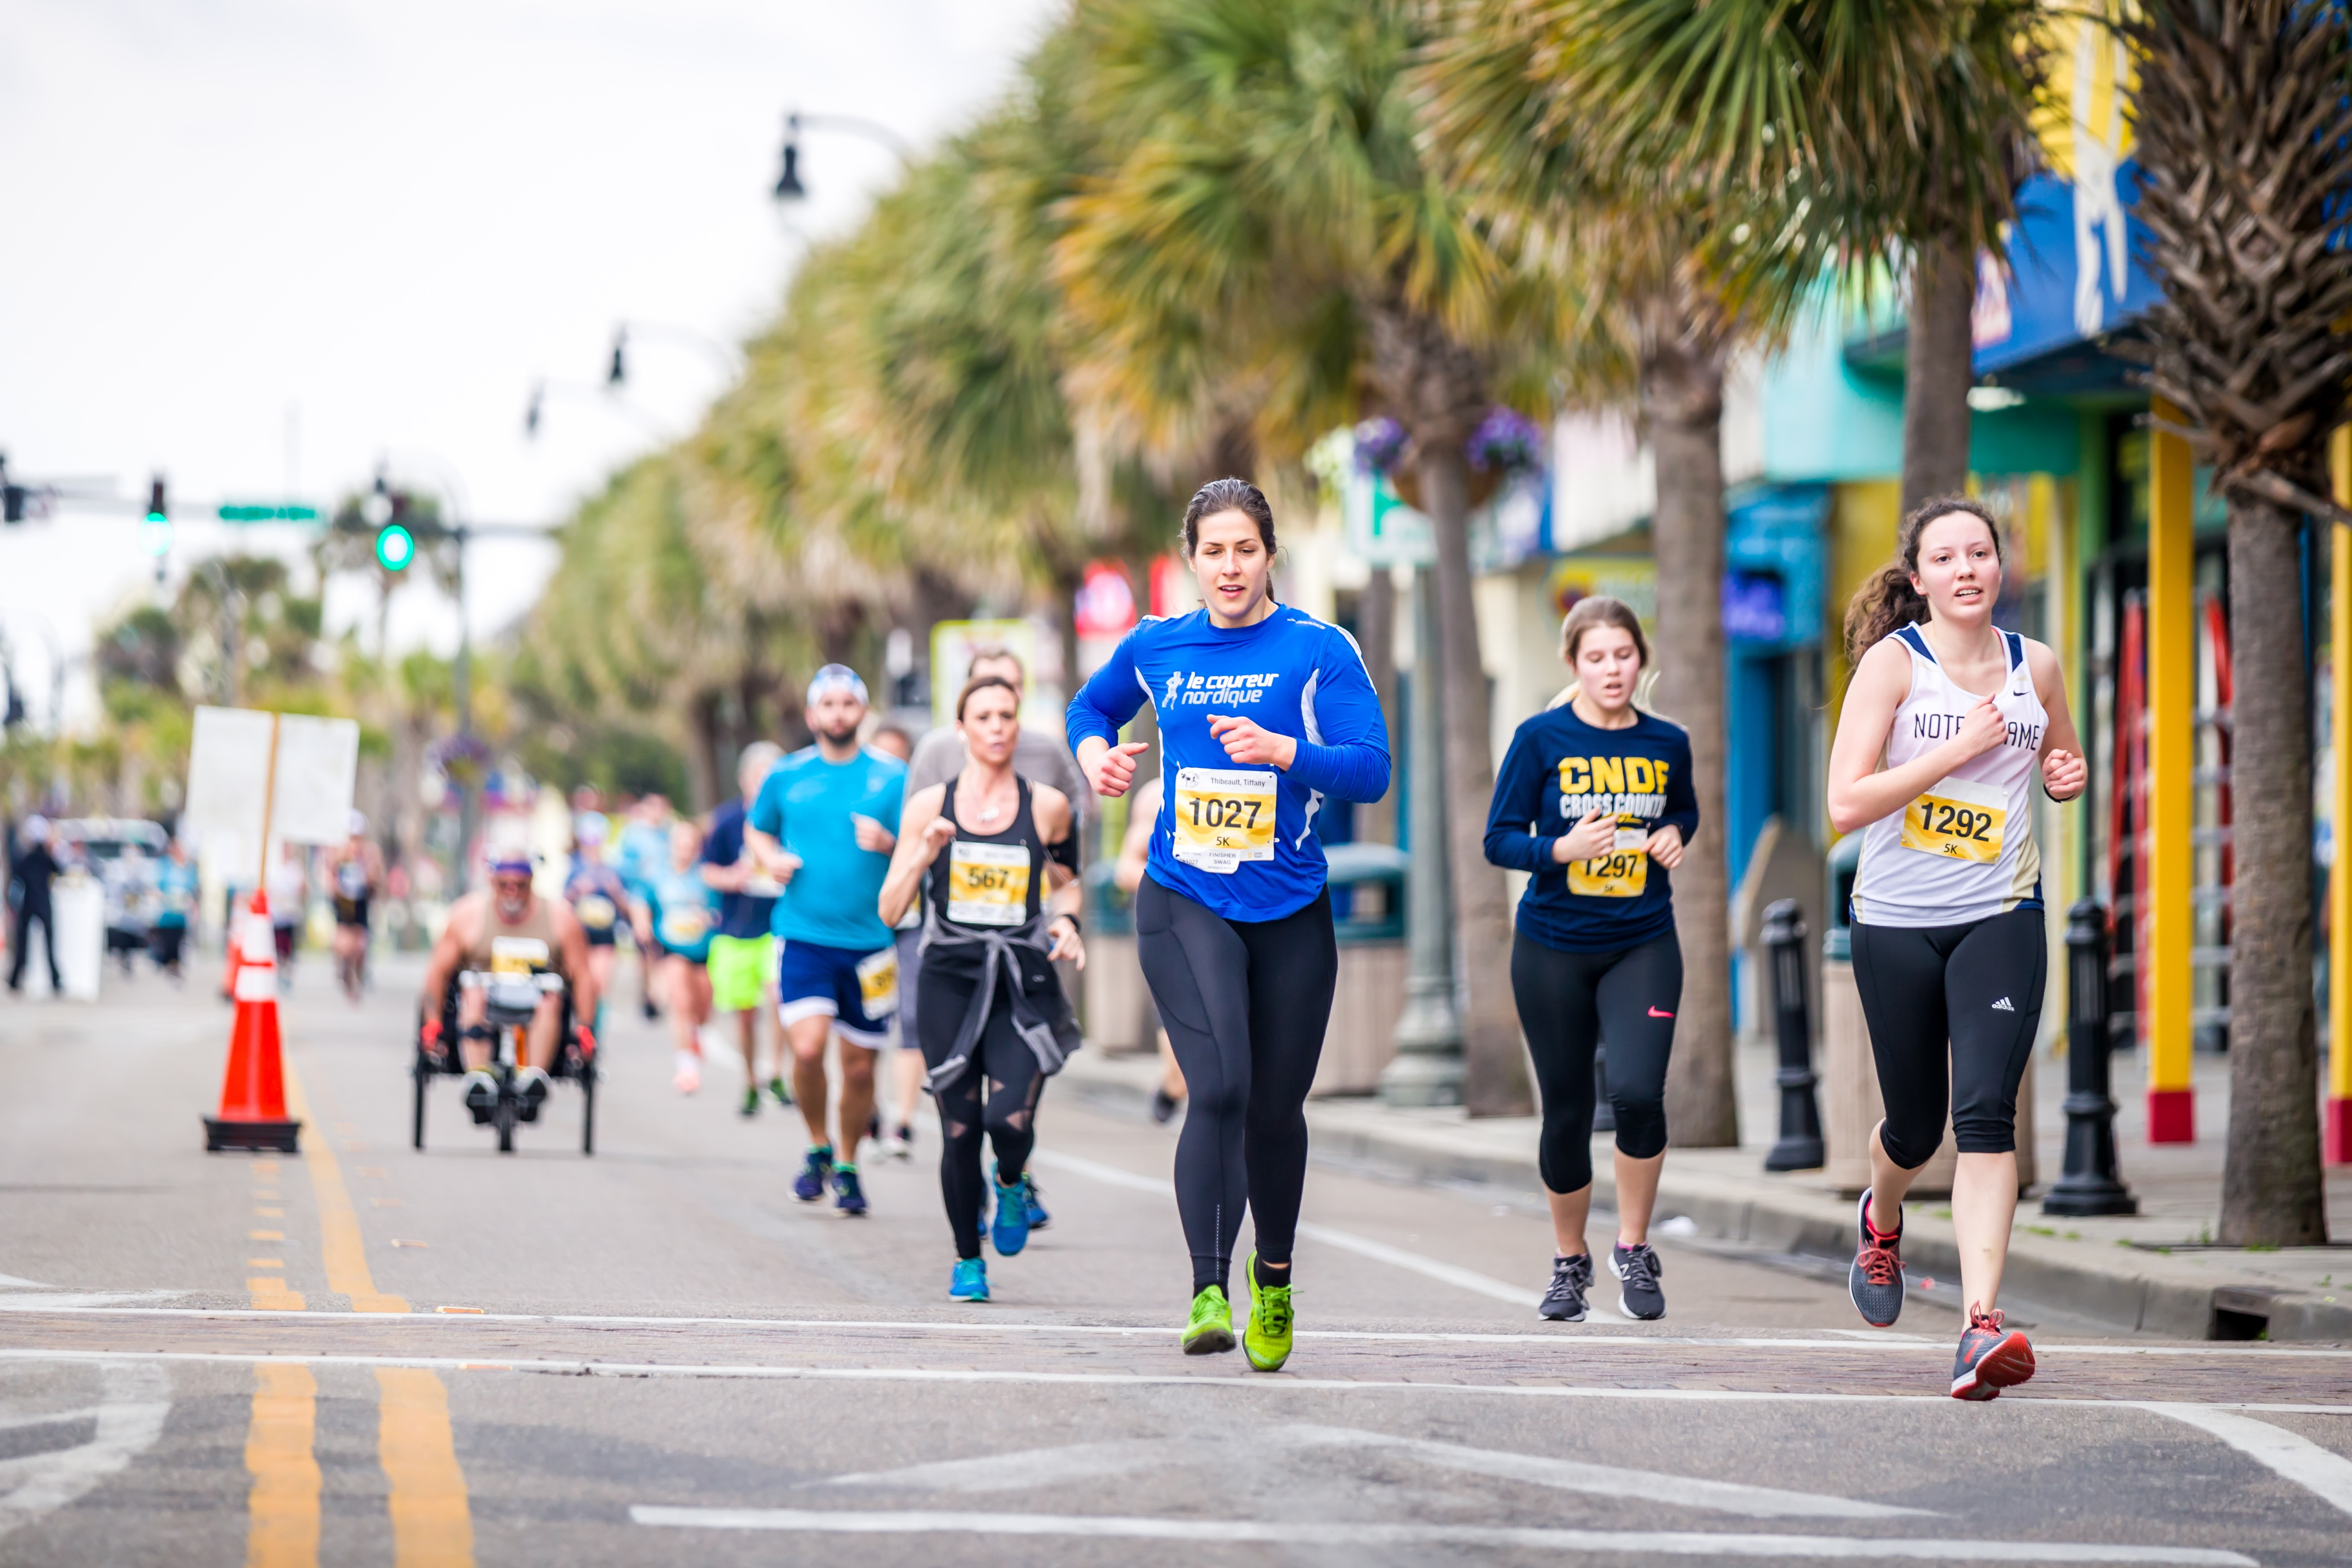
\includegraphics[width=\textwidth]{runners.jpg}
\end{center}

\end{frame}

\begin{frame}

\frametitle{Wie können wir gemessene Daten darstellen?}


\begin{tabular}{lll}
Teilnehmer*in   & Gewicht (kg)  &  5k Zeit (s)  \\
715 &	64.8 &	1875  \\
639 &	60.2 &	1538 \\
456 &	59 &	1645 \\
646 &	70.8 &	2129 \\
693 &	56.9 &	1676 \\
701 &	56.9 &	1793 \\
180 &	73.4 &	1956 \\
518 &	44.9 &	1539 \\
503 &	60.1 &	1606 \\
762 &	55.4 &	1808 \\
897 &	63.9 &	1917 \\
911 &	52 &	1791 \\
340 &	50.3 &	1705 \\
108 &	62.1 &	1721 \\
\end{tabular}



\end{frame}


\begin{frame}
%% Mittelwert, Standardabweichung, SEM
\frametitle{Wie können wir gemessene Daten darstellen?}

Zusammengefasste Statistiken (bei \(n\) Messwerten \(x_1, x_2, \dots, x_n\)):

\begin{itemize}
\item
Arithmetischer Mittelwert (``Wie groß ist der Wert im Durchschnitt?'')
\[
\bar{x} =  \frac{x_1 + x_2 + \dots + x_n}{n} = \frac{\sum_{i=1}^n x_i}{n}
\]
\pause
\item
Standardabweichung (``Wie stark variieren die Messwerte?'')
\[
s = \sqrt{\frac{\sum_{i=1}^n (x_i-\bar{x})^2}{n-1}}
\]
\pause
\item
Standardfehler des arithmetischen Mittelwerts (``Wo liegt der echte Mittelwert wahrscheinlich?'')
\[
SAM = \frac{s}{\sqrt{n}}
\]
\end{itemize}


\end{frame}

 
\begin{frame}
\frametitle{Berechnen Sie das arithmetische  Mittel des Gewichts}

\begin{tabular}{lll}
Teilnehmer*in   & Gewicht (kg)  &  5k Zeit (s)  \\
715 &	64.8 &	1875  \\
639 &	60.2 &	1538 \\
456 &	59 &	1645 \\
646 &	70.8 &	2129 \\
693 &	56.9 &	1676 \\
701 &	56.9 &	1793 \\
180 &	73.4 &	1956 \\
518 &	44.9 &	1539 \\
503 &	60.1 &	1606 \\
762 &	55.4 &	1808 \\
897 &	63.9 &	1917 \\
911 &	52 &	1791 \\
340 &	50.3 &	1705 \\
108 &	62.1 &	1721 \\
\end{tabular}



\end{frame}

\begin{frame}
\frametitle{Berechnen Sie das arithmetische  Mittel des Gewichts}

\[
\bar{x} = 59.33571\,\text{kg}
\]


\pause

Echt?

\pause

Ist es sinnvoll, das mittlere Gewicht auf \SI{10}{\milli\gram} genau anzugeben?  \pause Nein! Kleiner Exkurs:


\end{frame}



%% %% Messunsicherheit

\begin{frame}
\makebox[\linewidth]{
\includegraphics[page=29,width=\textwidth]{Walter.pdf}}
\end{frame}

\begin{frame}
\makebox[\linewidth]{
\includegraphics[page=30,width=\textwidth]{Walter.pdf}}
\end{frame}

\begin{frame}
\makebox[\linewidth]{
\includegraphics[page=37,width=\textwidth]{Walter.pdf}}
\end{frame}


%% %% Messunsicherheit
\begin{frame}
\frametitle{Fehlerfortpflanzung}

Sehr einfache Faustregel:

Das Ergebnis sollte nicht mit mehr Präzision angegeben werden als die ursprünglichen Daten. 

\pause

\[
\bar{x} = 59.3\,\text{kg}
\]

\end{frame}



%% Funktionsgraphen
\begin{frame}
\frametitle{Funktionsgraphen}

Wir können  gemessene Daten auch graphisch darstellen:

\begin{center}
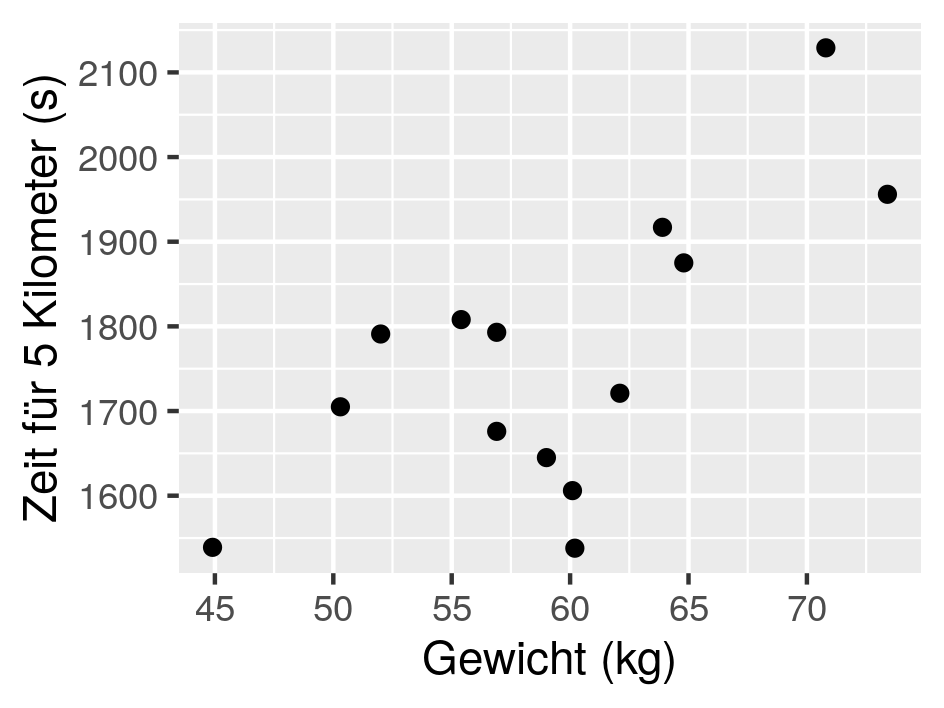
\includegraphics{zeit_vs_gewicht.png}
\end{center}

\end{frame}


\begin{frame}
\frametitle{Funktionsgraph}

Darstellung eines Wertes (y) in Abhängigkeit von einem anderen Wert (x). Dabei kann es für jeden x-Wert nur einen y-Wert geben. 

\begin{center}
\includegraphics<1>{zeit_vs_gewicht_regression.png}
\includegraphics<2>{function.png}
\end{center}

\end{frame}


%% Ableitung,
\begin{frame}
\frametitle{Differenzieren}

Um die \emph{Veränderung} eines Funktionsgraphen an jedem Punkt zu ermitteln, wird differenziert.

\begin{center}
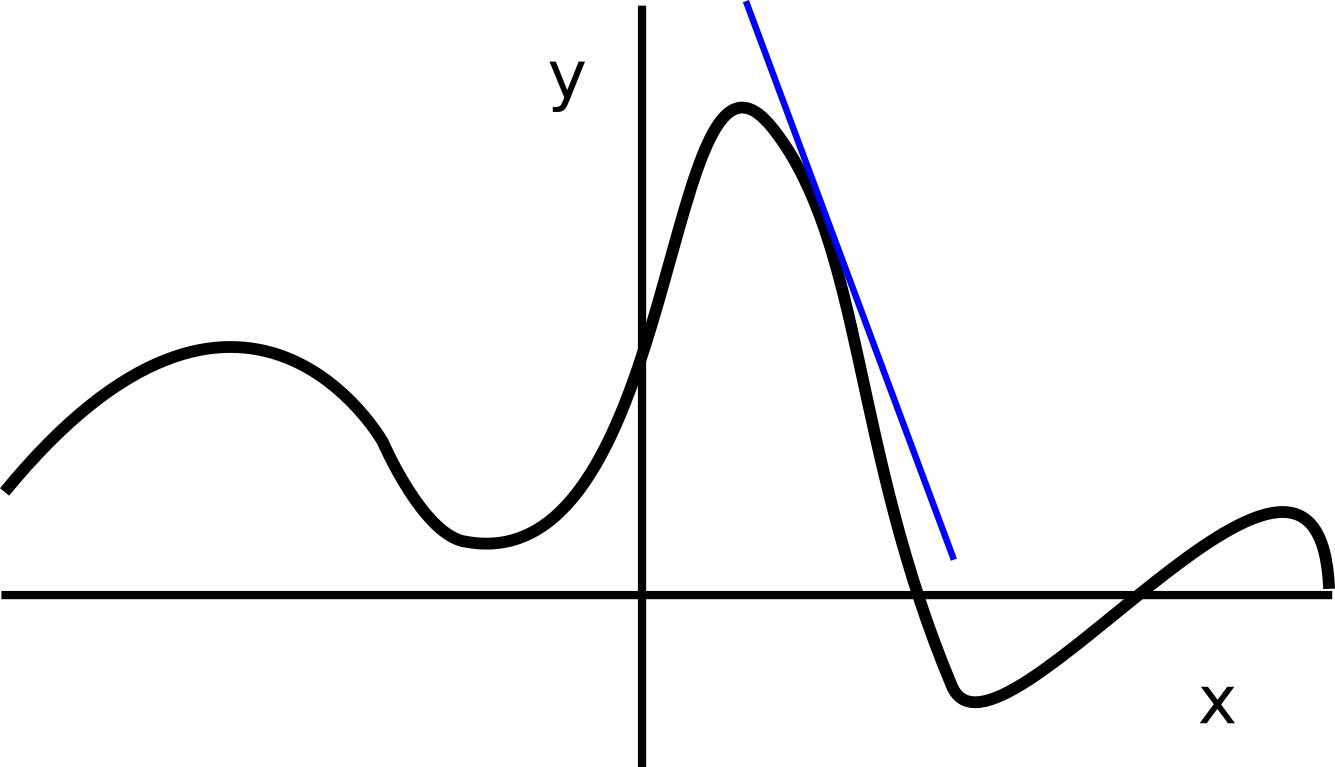
\includegraphics{function_diff.png}
\end{center}


\end{frame}


\begin{frame}
\frametitle{Differenzieren}

Um die \emph{Fläche unter} einem Funktionsgraphen zu ermitteln, wird integriert.

\begin{center}
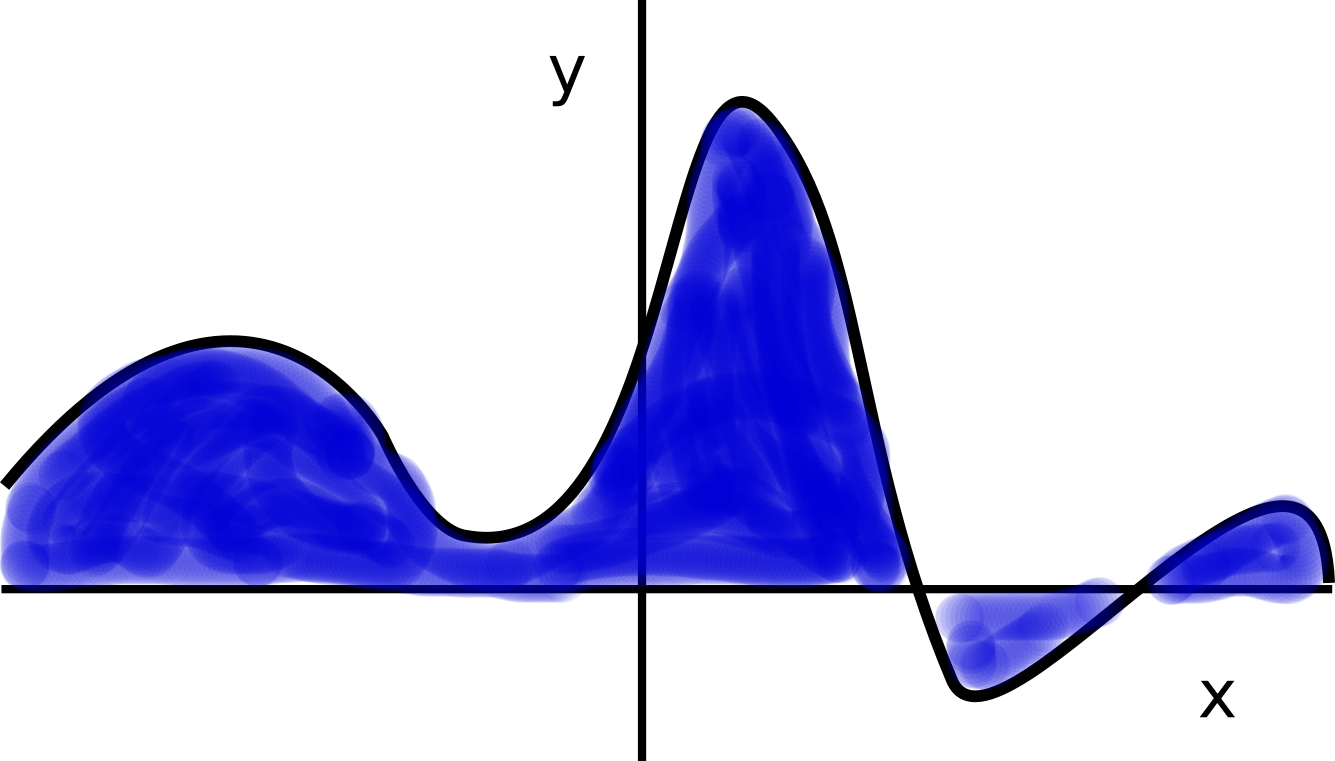
\includegraphics{function_int.png}
\end{center}


\end{frame}





%% Glockenkurve
\begin{frame}
\frametitle{Histogramme}

Graphische Darstellung einer Messreihe, die zeigt, wie Werte verteilt sind. Zurück zum früheren Beispiel:


\begin{center}
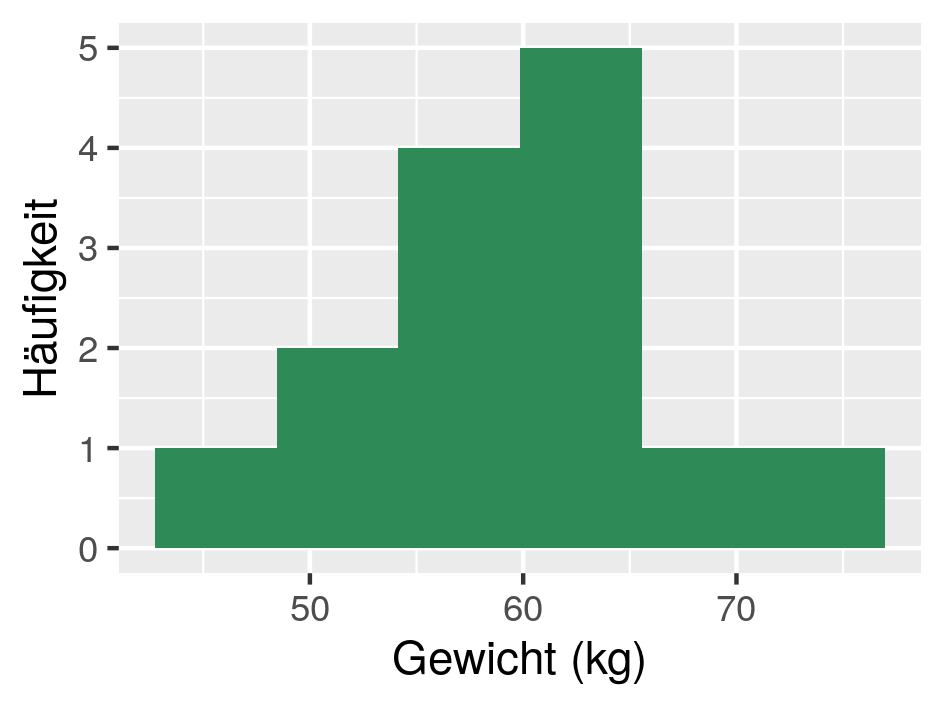
\includegraphics{histogram.png}
\end{center}


\end{frame}

\begin{frame}
\frametitle{Gaußsche Glockenkurve}

Solche Histogramme sind oft ``glockenförmig'' (symmetrisch, mit einem Gipfel beim Mittelwert). Solche Daten sind ``normalverteilt'' und folgen der 68-95-99.7-Regel.


\begin{center}
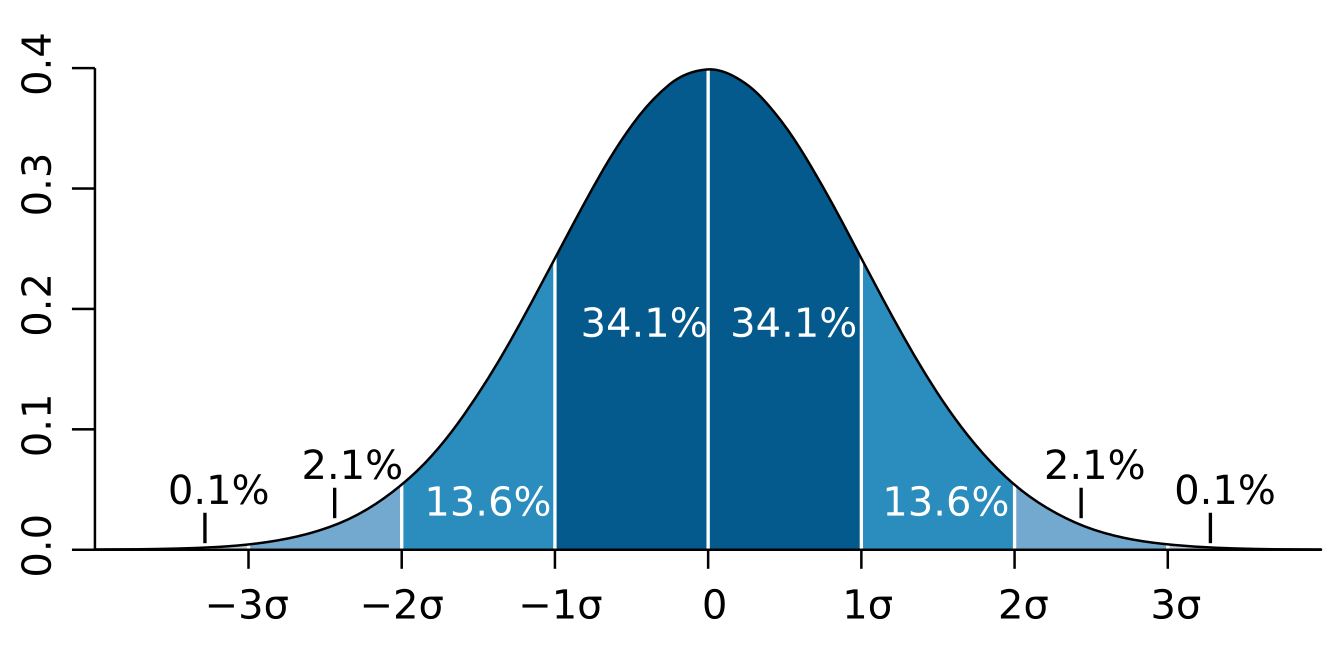
\includegraphics[width=\textwidth]{empirical_rule.png}
\end{center}





\end{frame}

%% Glockenkurve waruuum?
\begin{frame}
\frametitle{Aber wie oft sind Daten normalverteilt?}

Erstaunlich oft! Normalverteilungen kommen oft natürlich zustande, wenn eine Größe eine Kombination (z.B. Summe) aus anderen zufälligen Größen ist. Anschauliches Beispiel: Summe im Würfelspiel:

\begin{center}
\includegraphics<1>[width=0.8\textwidth]{onedie.png}
\includegraphics<2>[width=0.8\textwidth]{twodice.png}
\includegraphics<3>[width=0.8\textwidth]{fivedice.png}
\end{center}



\end{frame}

\begin{frame}
\frametitle{Beispiel: Typische IMPP Frage}

Für ein sportmedizinisches Experiment wird die Körpergröße von olympischen Basketballspielern  gemessen. Die gemessenen Größen sind annähernd normalverteilt, mit einer  Durchschnittsgröße von \SI{198}{\centi\meter}  und einer Standardabweichung von 6 cm. Welcher Anteil der Spieler ist größer als \SI{210}{\centi\meter}?


\begin{description}
\item[A] \(68\,\%\) 
\item[B] \(34,1\,\%\)
\item[C] \(13,6\,\%\)
\item[D] \(5\,\%\)
\item[E] \(2,2\,\%\)
\end{description}

\end{frame}

\begin{frame}
\frametitle{Beispiel: Typische IMPP Frage}

\begin{center}
\includegraphics<1>[width=\textwidth]{empirical_rule.png}
\includegraphics<2>[width=\textwidth]{empirical_rule_example_Part1.png}
\includegraphics<3>[width=\textwidth]{empirical_rule_example_Part2.png}
\includegraphics<4>[width=\textwidth]{empirical_rule_example_Part3.png}
\end{center}


\end{frame}


\section{Rechnen}

%% Exponential
\begin{frame}
\frametitle{Exponentialfunktion}

Die Exponentialfunktion beschreibt Vorgänge, bei denen sich y-Werte im selben x Intervall jeweils um den selben Faktor vervielfachen. 

\[
y  = a^x
\]


(wo die Basis \(a\) eine Konstante ist)





\end{frame}

\begin{frame}
\frametitle{Exponentialfunktion}

 In der Biologie/Medizin meistens in der Form:

\[
y = y_0 e^{kt}
\]

Wobei:

\begin{tabular}{ll}
\(y_0\) & Startwert \\
\(e\)   & Euler'sche Konstante (\(\sim 2.72\))  \\
\(t\)   & Zeit \\
\(k\)   & Konstante (exponentielles Wachstum für positives k, \\
        & exponentieller Zerfall für negatives k) \\
\end{tabular}


\end{frame}


\begin{frame}
\frametitle{Beispiel: Übertragbare Krankheit}

% Beispiel: Infektionskrankheiten 
\begin{columns}[c]
\begin{column}{5cm}

\[
y = y_0 e^{kt}
\] 


\begin{center}

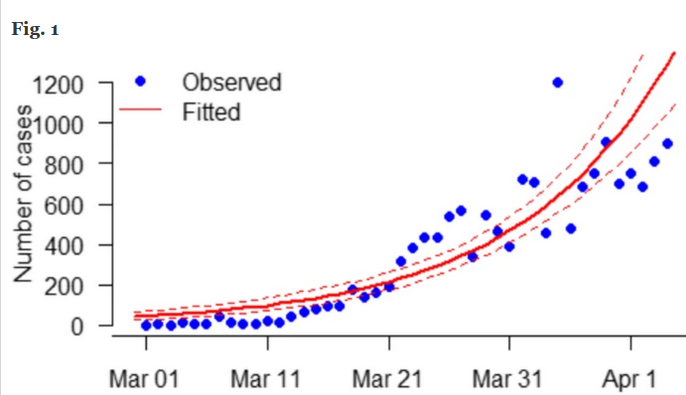
\includegraphics[width=\textwidth]{Covid19_Africa.png}
\end{center}



\end{column}
\begin{column}{5cm}

\begin{center}
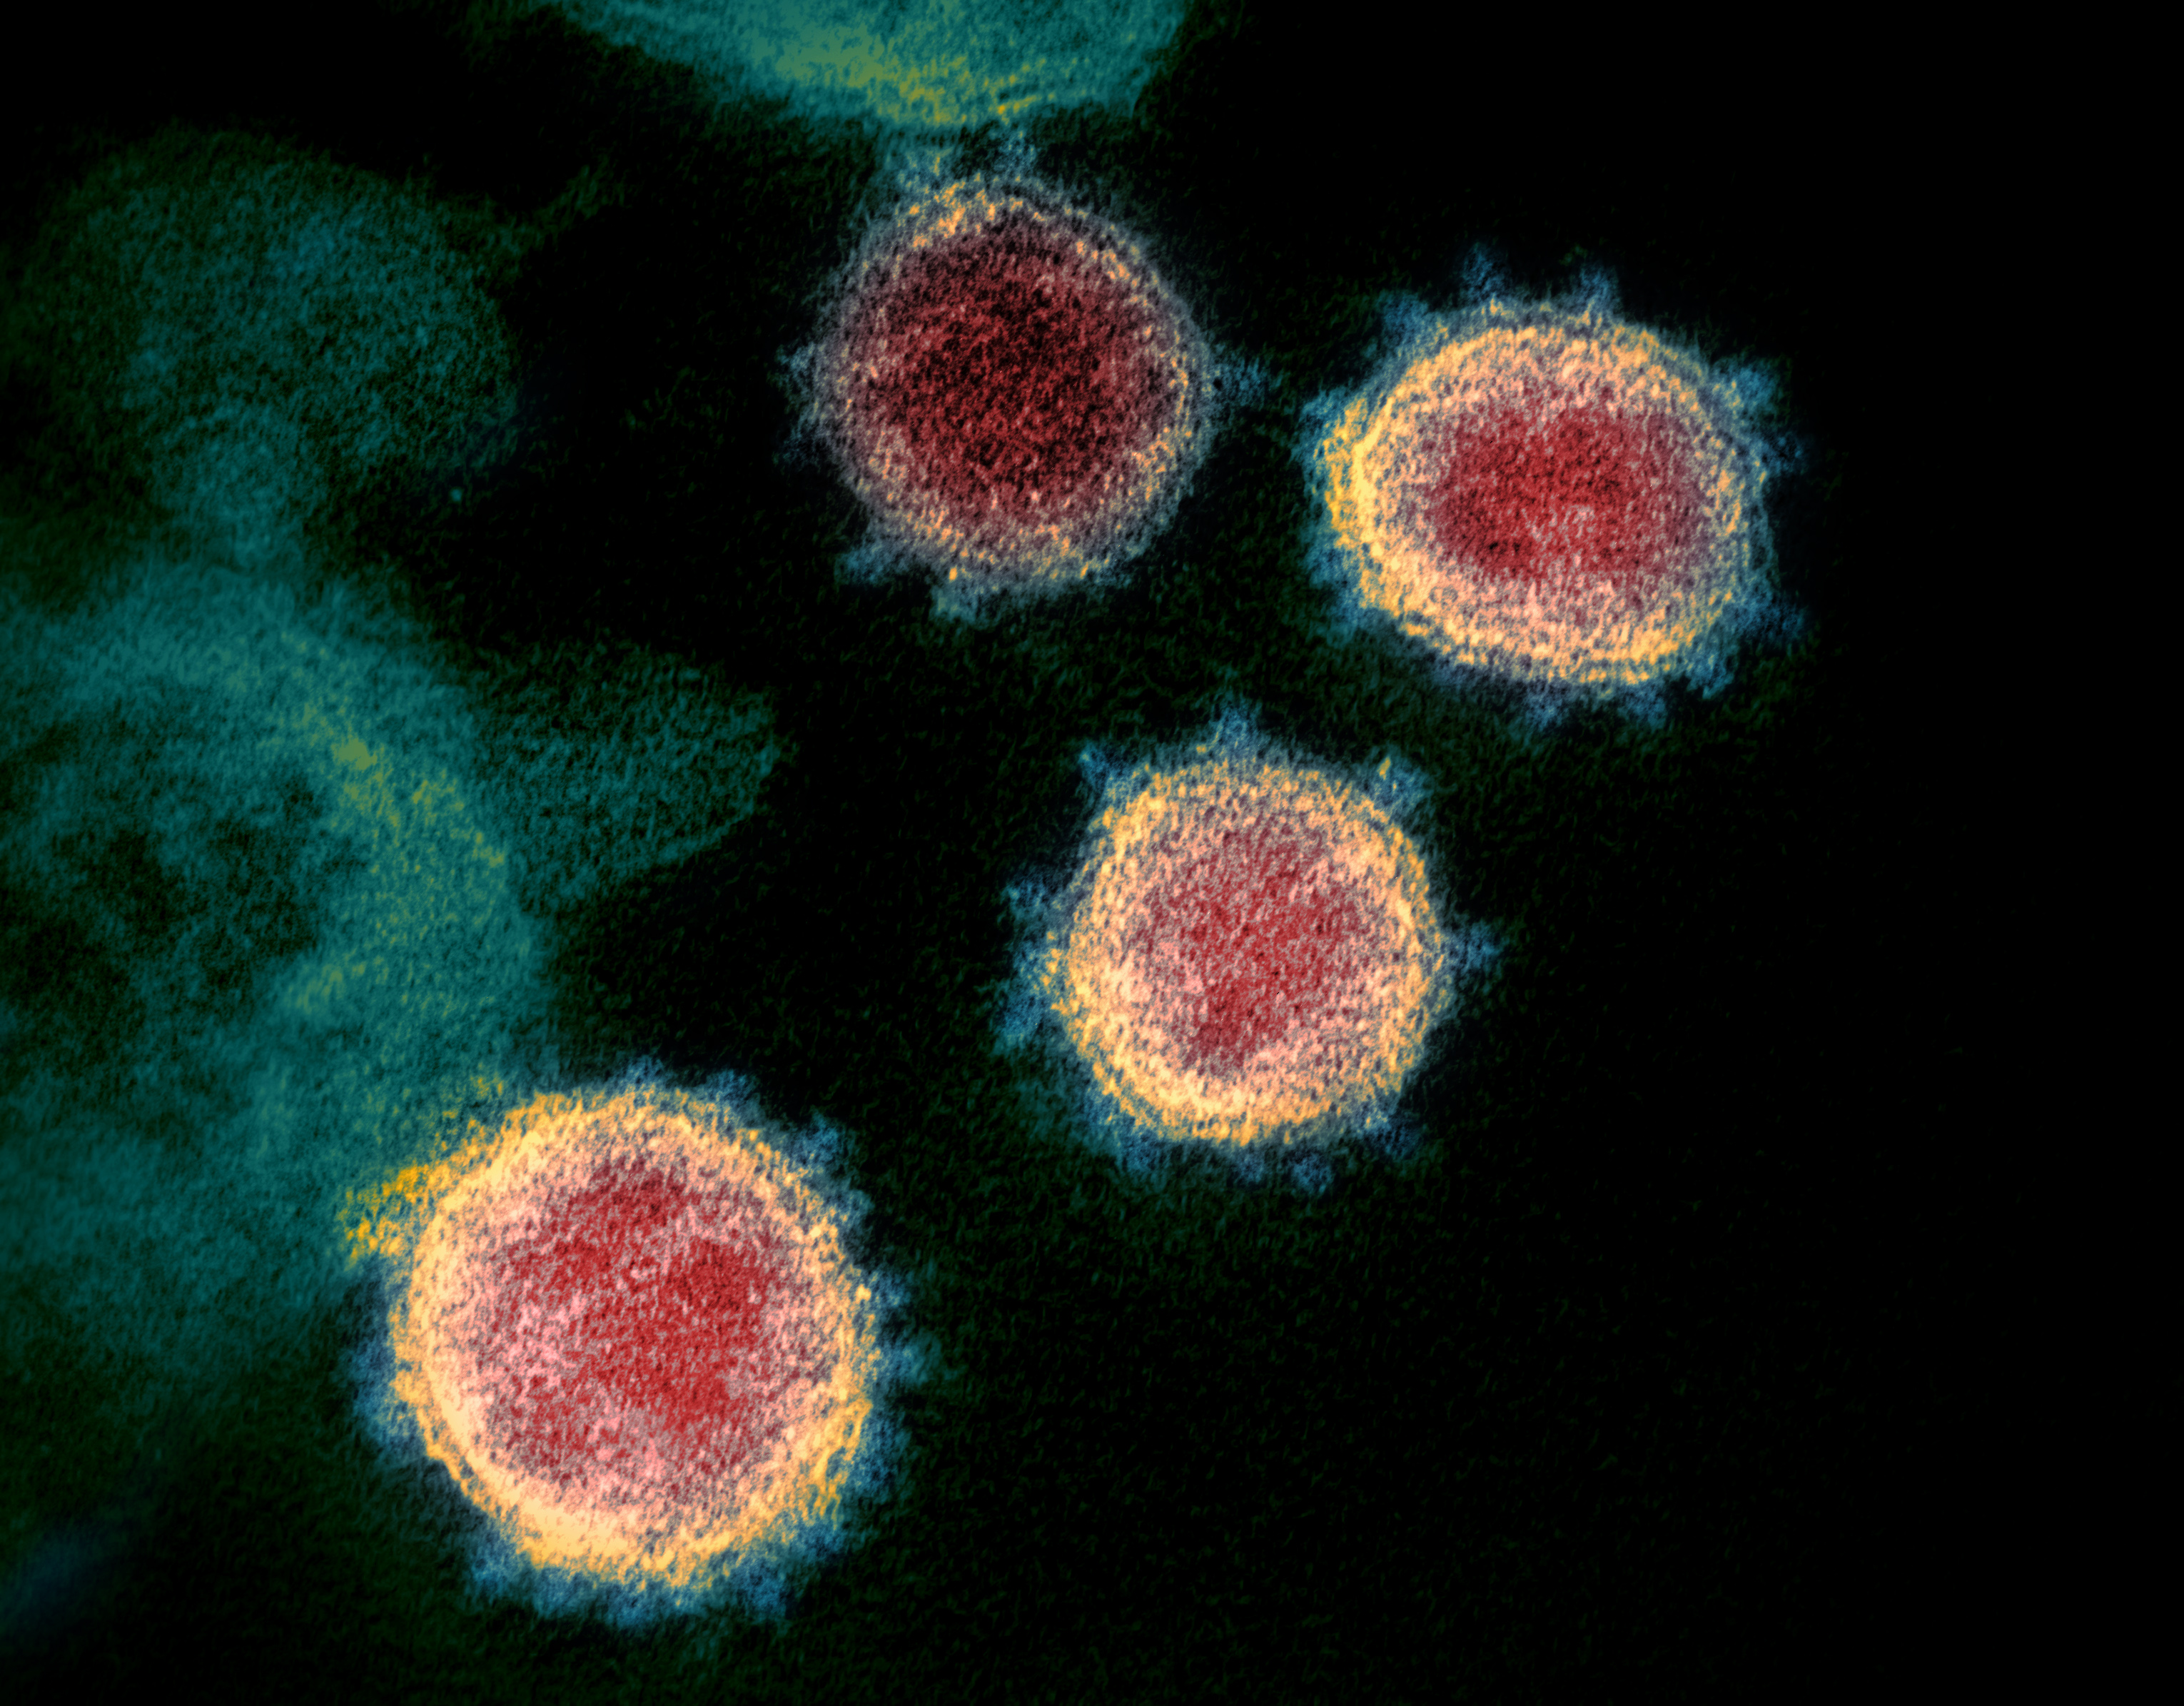
\includegraphics[width=\textwidth]{SARS-CoV-2.jpg}
\end{center}


\end{column}
\end{columns}


\end{frame}

\begin{frame}
\frametitle{Beispiel: Übertragbare Krankheit}

% Beispiel: Infektionskrankheiten 
\begin{columns}[c]
\begin{column}{5cm}

\[
y = y_0 e^{kt}
\] 


\begin{center}

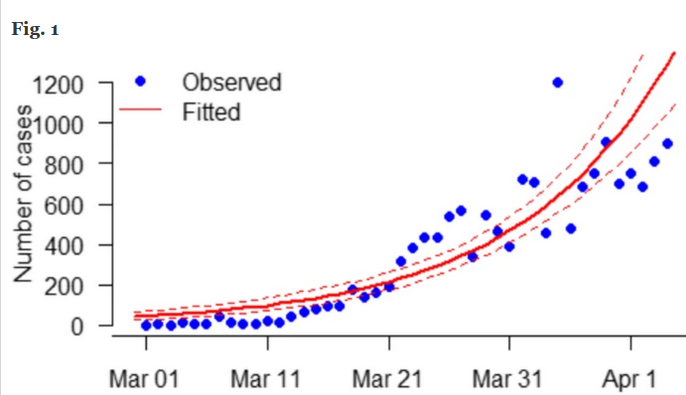
\includegraphics[width=\textwidth]{Covid19_Africa.png}
\end{center}



\end{column}
\begin{column}{5cm}

Wie ändert sich die Gleichung, wenn wir:

\begin{itemize}
\item
Schutzmasken verwenden? 
\item
Zu Beginn der Pandemie Erkrankte isolieren?
\end{itemize}


\end{column}
\end{columns}


\end{frame}



\begin{frame}
\frametitle{Logarithmus}

Logarithmen sind ``das Gegenteil'' von Exponentialrechnungen

Wenn 

\[
y = a^x
\]

Dann

\[
log_a(y) = x
\]


``Der Logarithmus von y auf der Basis a ist x'' 


\pause

Häufig verwendete Basen: 

\begin{itemize}
\item
10 (geschrieben log\textsubscript{10}, lg, log)
\item
e (``natürlicher Logarithmus'', geschrieben ln, log)
\end{itemize}

\end{frame}


\begin{frame}
\frametitle{OK \dots}

\pause

Aber warum????

\begin{center}
\includegraphics<2>[width=\textwidth]{confused_guy.jpg}
\end{center}

\pause

Weil Logarithmen das Rechnen einfacher machen!

Um Zahlen zu multiplizieren, muss man nur die Logarithmen addieren.  \\
Um Exponentiale zu berechnen, muss man nur die Logarithmen multiplizieren. \\

\pause

Und: Weil Logarithmen oft "natürlich" vorkommen.

\end{frame}

\begin{frame}

\frametitle{Beispiel: Wahrnehmung}

Ob wir einen Unterschied in der Reizstärke wahrnehmen können, hängt oft davon ab, wie stark der Reiz schon ist (Mehr dazu im 4. Semester Physio!)




\begin{columns}[c]
\begin{column}{5cm}

\begin{center}
    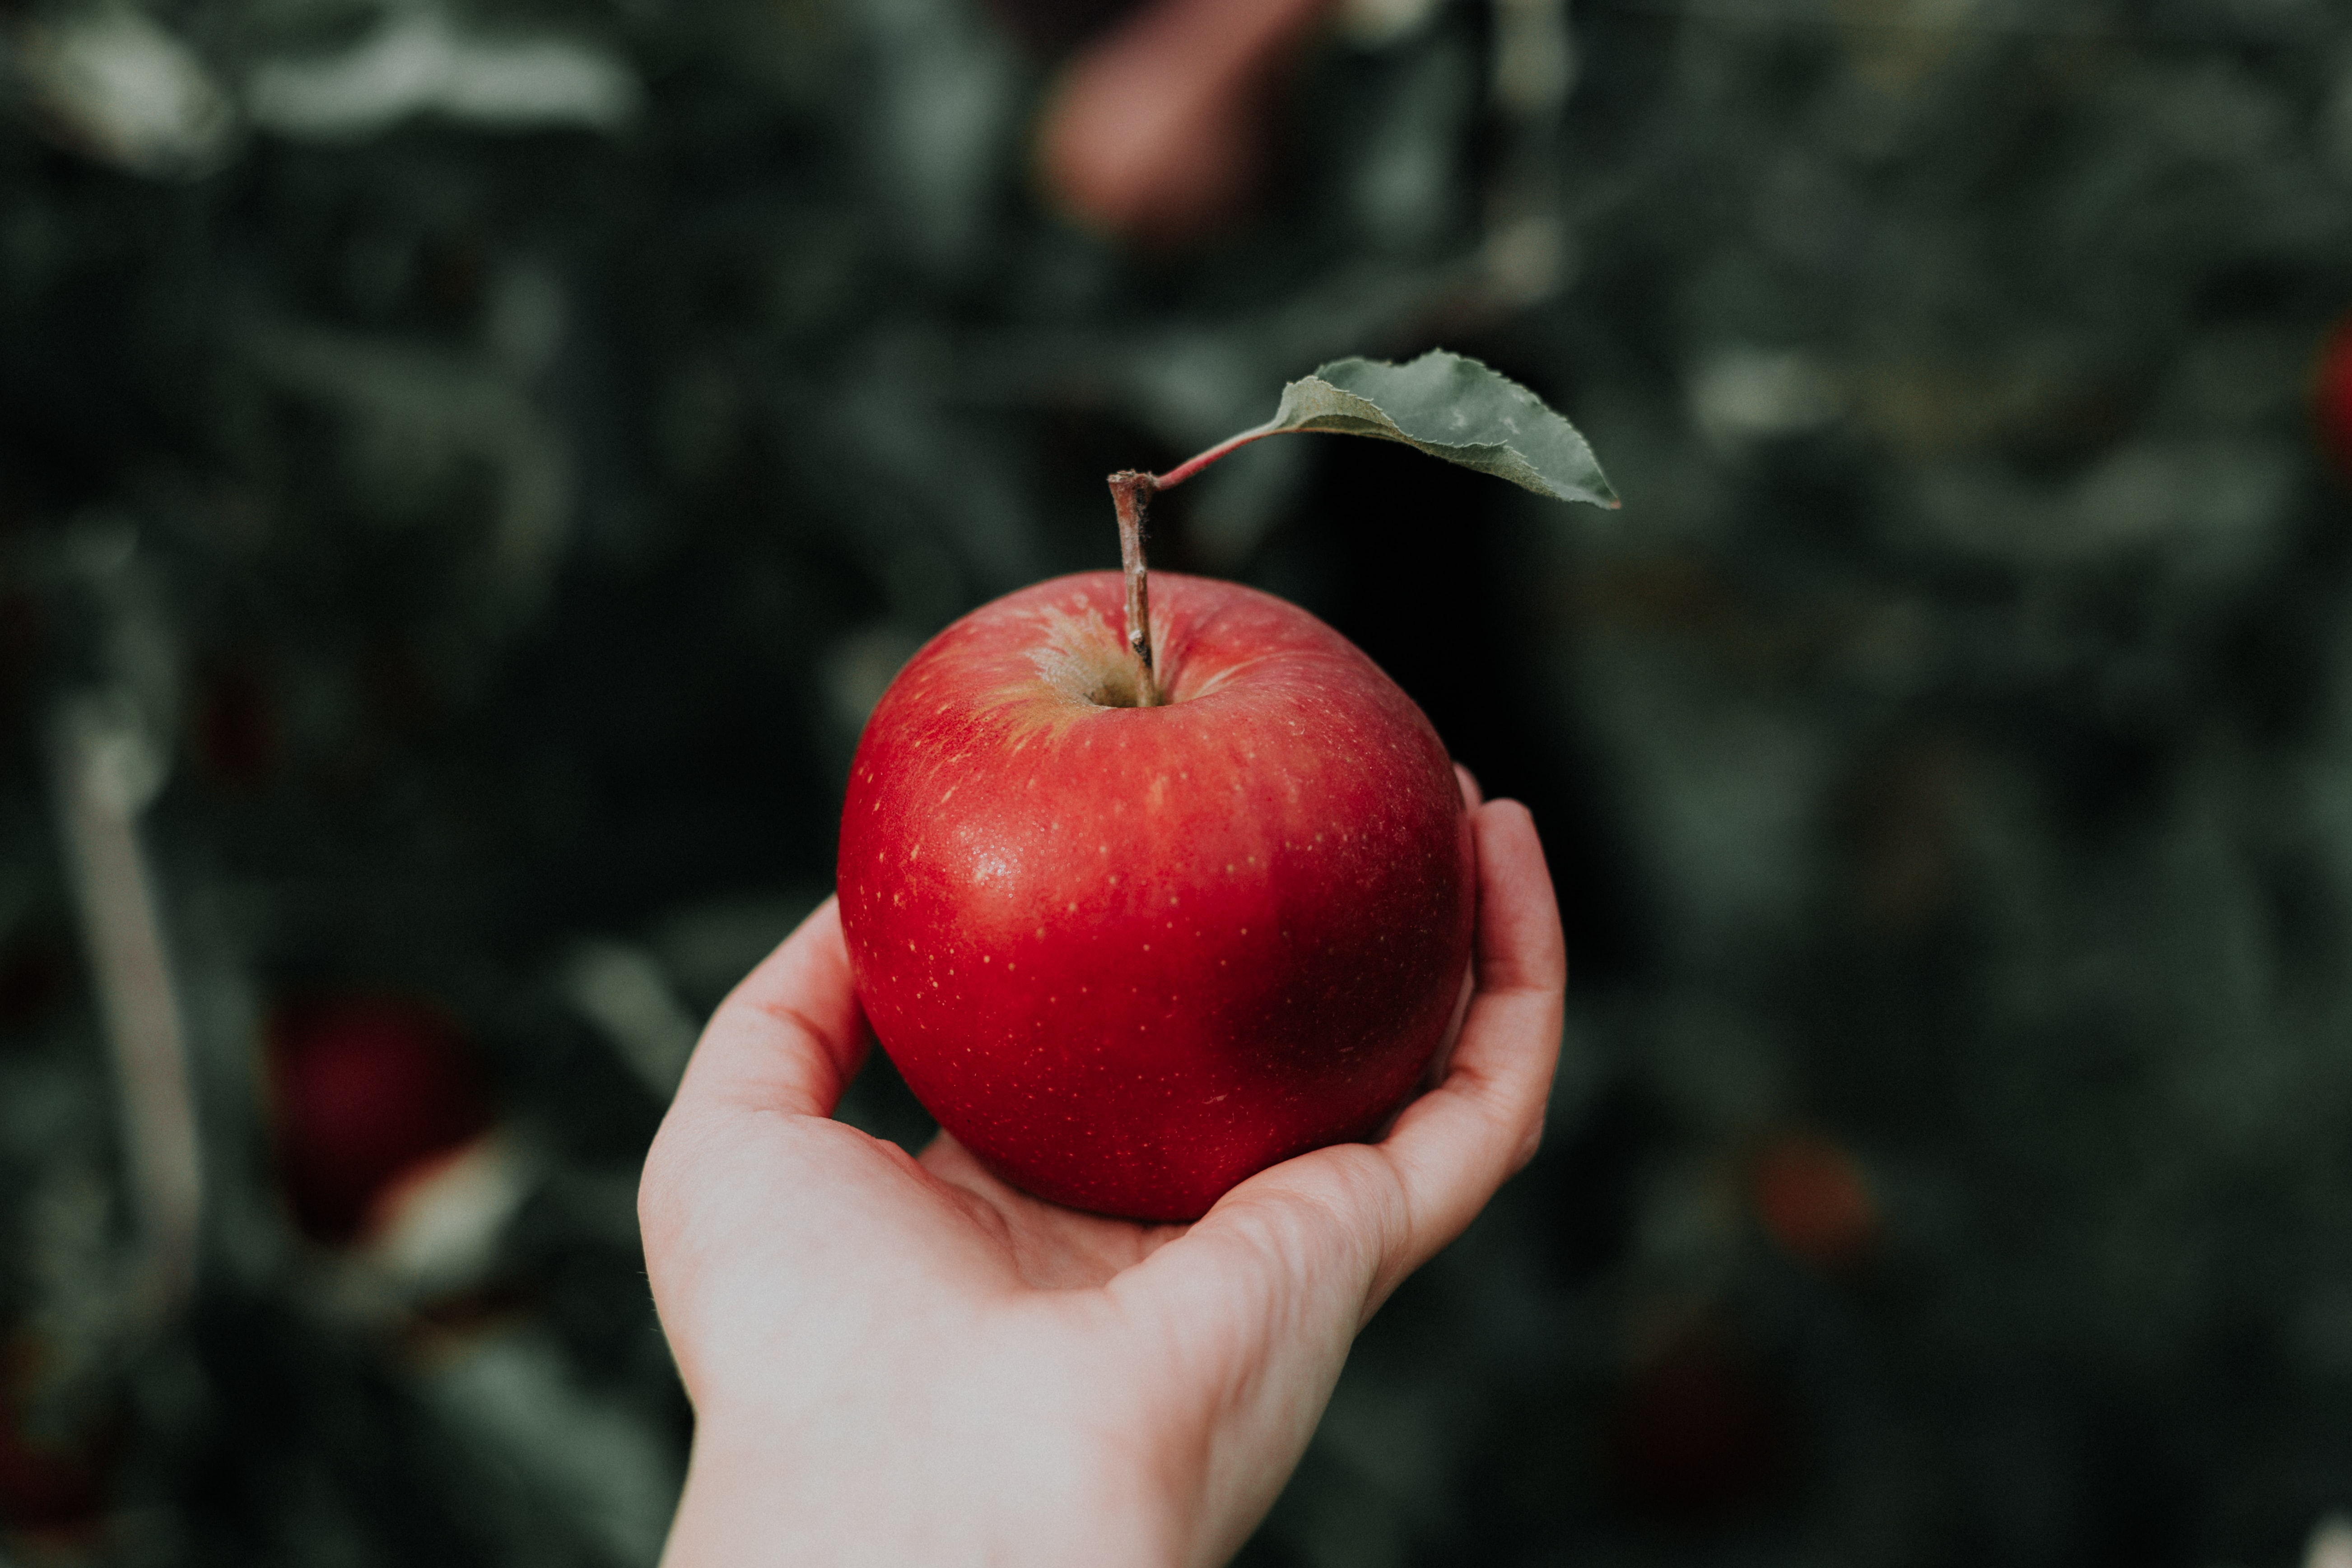
\includegraphics[width=\textwidth]{priscilla-du-preez-CoqJGsFVJtM-unsplash.jpg}
        
\end{center}

    
\end{column}
\pause
\begin{column}{5cm}
\begin{center}

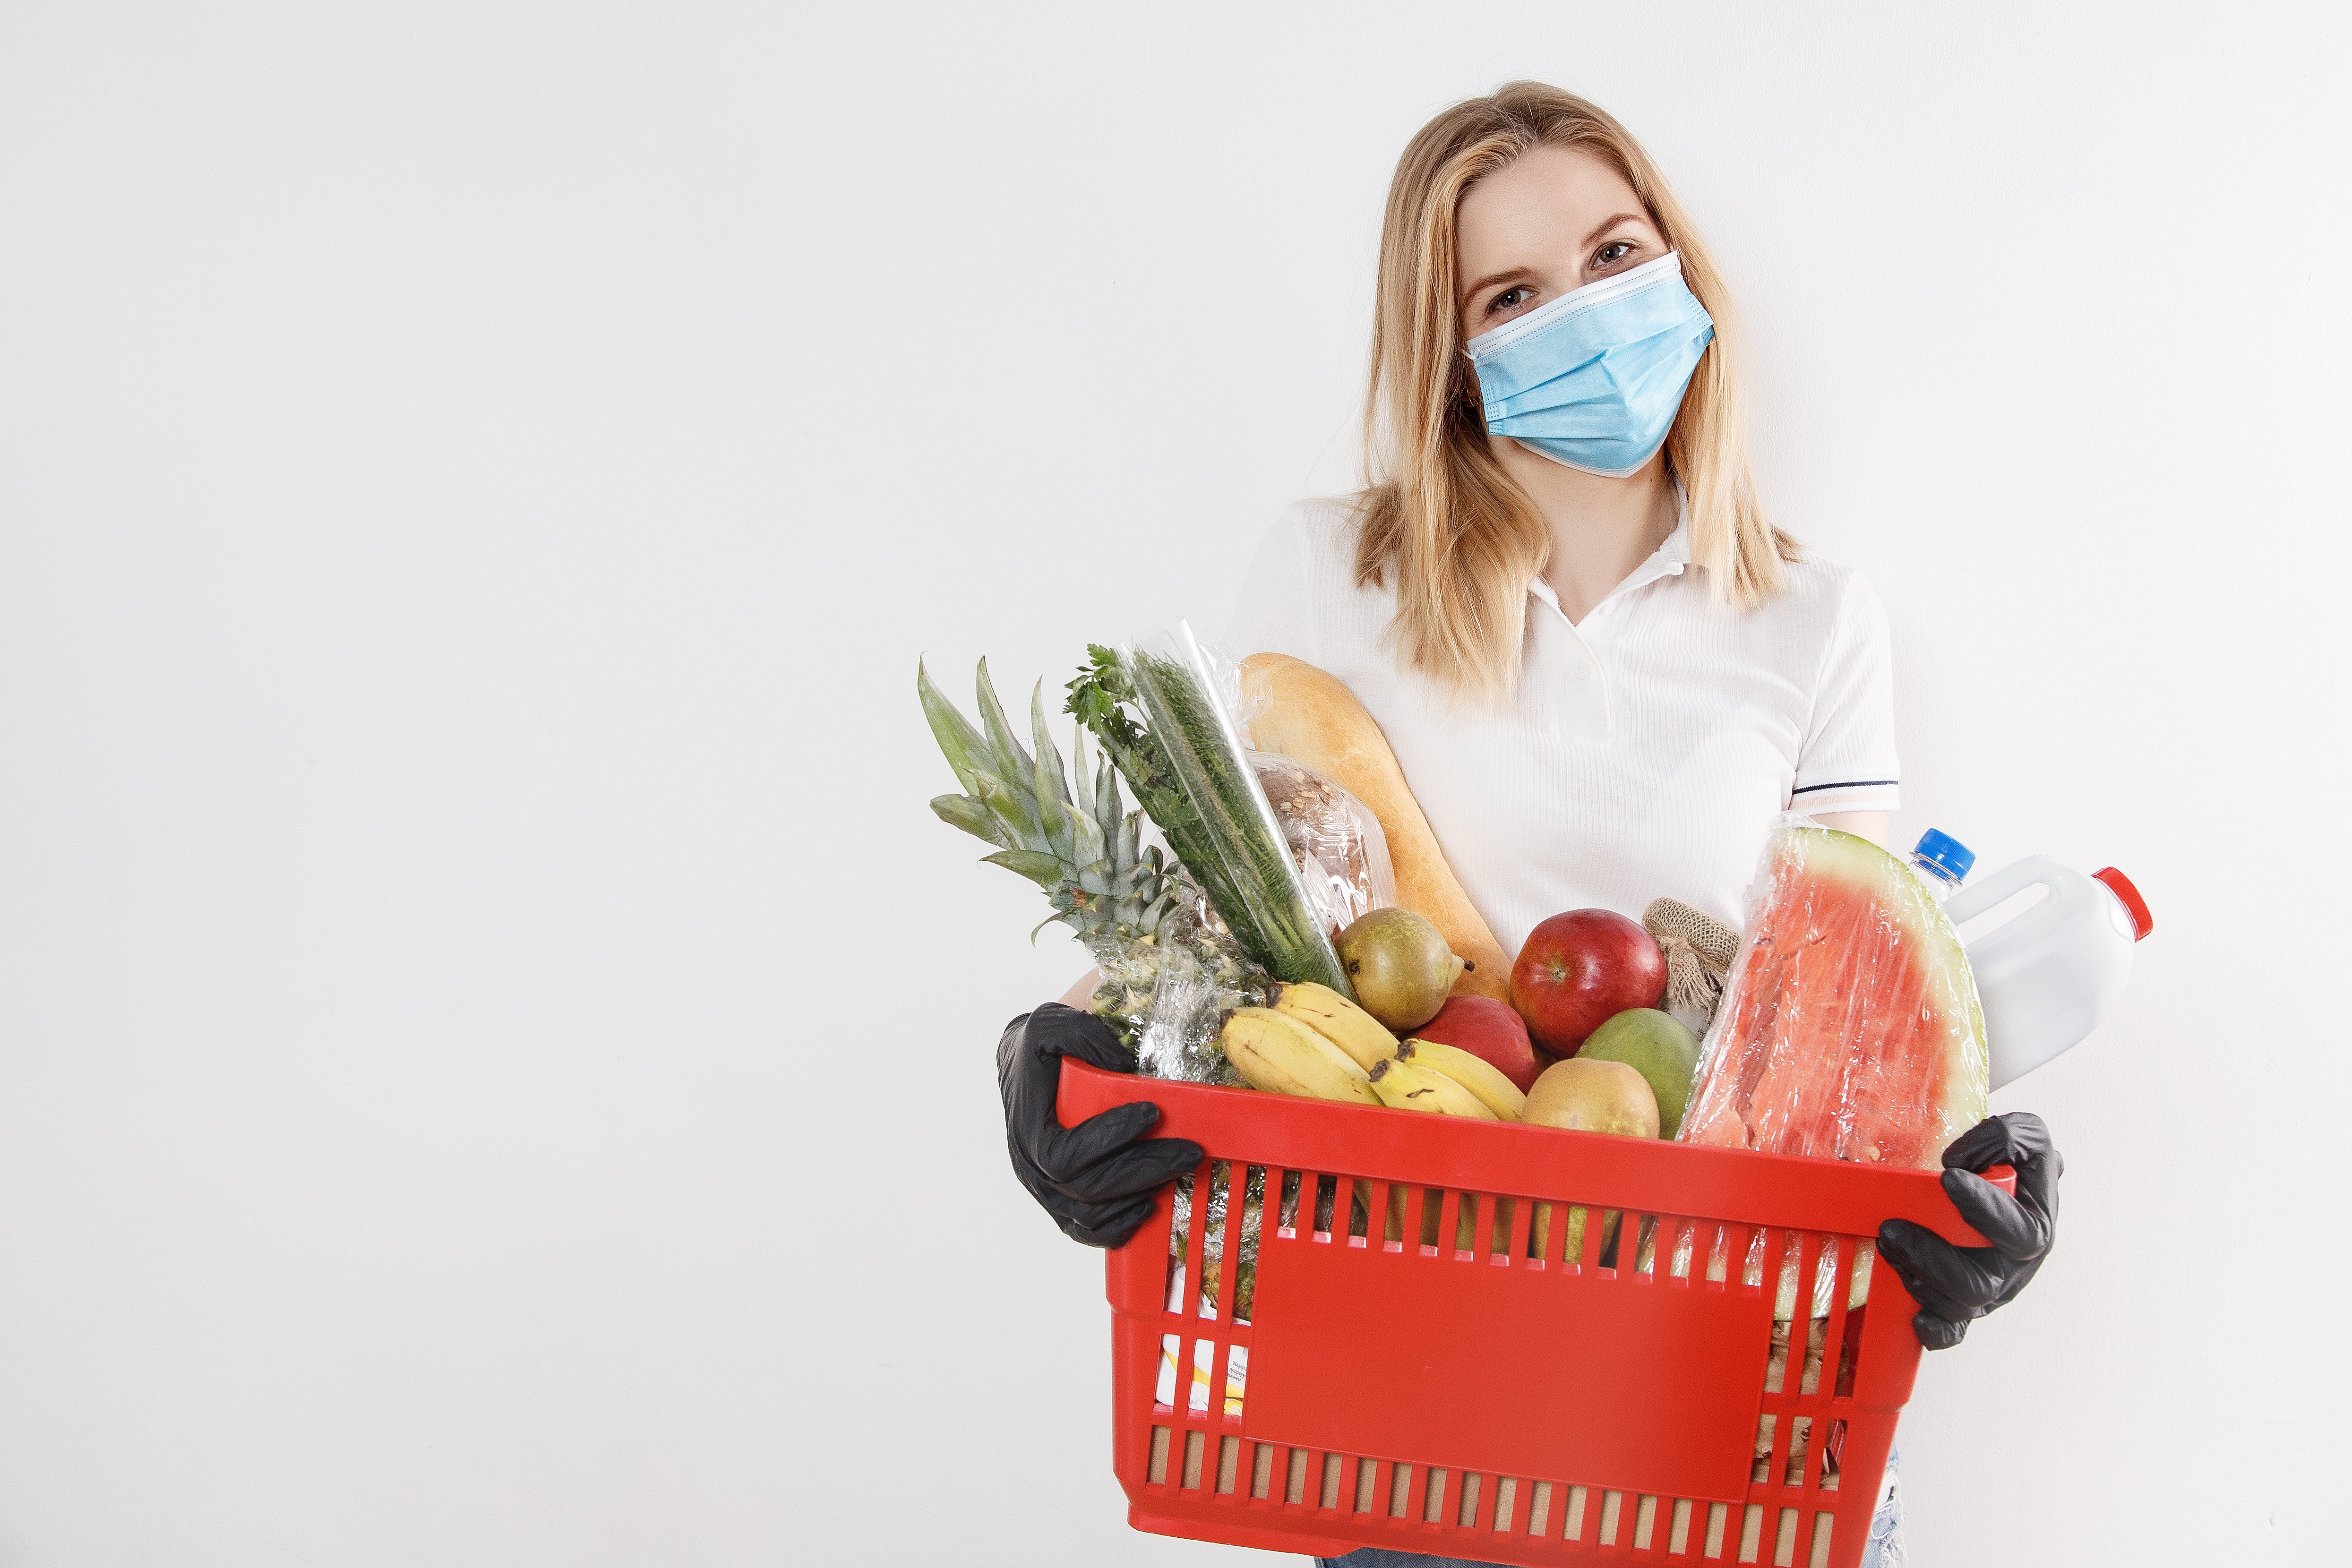
\includegraphics[width=\textwidth]{liuba-bilyk-wU_TbWqdPJI-unsplash.jpg}
\end{center}

    
\end{column}
    
\end{columns}

\begin{center}
    
\end{center}




\end{frame}


\begin{frame}

\frametitle{Beispiel: Wahrnehmung}

\begin{center}
    \includegraphics<1>[width=0.8\textwidth]{weber_fechner.png}
    \includegraphics<2>[width=0.8\textwidth]{weber_fechner_log_scale.png}

\end{center}

\end{frame}

%% Vektoren

\begin{frame}
\frametitle{Vektoren}

Einzelne Zahlen (Skalare) können Größe, Gewicht, Blutzuckerspiegel etc. beschreiben.  Aber manchmal brauchen Paare oder Tripel (oder mehr) Zahlen gemeinsam, um z.B. eine Position im Raum zu bestimmen. Das sind Vektoren. \\


\begin{center}
\includegraphics<1>[width=0.6\textwidth]{vectors.png}
\includegraphics<2>[width=0.6\textwidth]{vectors_additon.png}
\end{center}



\end{frame}


\begin{frame}
\frametitle{Vektoren}

Derselbe Punkt kann beschrieben werden durch einen Winkel und eine Länge


\begin{center}
\includegraphics<1>[width=0.6\textwidth]{vectors.png}
\includegraphics<2>[width=0.6\textwidth]{vectors_winkel.png}
\end{center}



\end{frame}



%% Trig Funktionen
\begin{frame}
\frametitle{Trigonometrische Funktionen}

Trigonometrische Funktionen beschreiben Winkel. Am einfachsten zu sehen, indem wir den Winkel in einen \emph{Einheitskreis} einzeichnen (Länge der Hypotenuse = 1)

\begin{center}
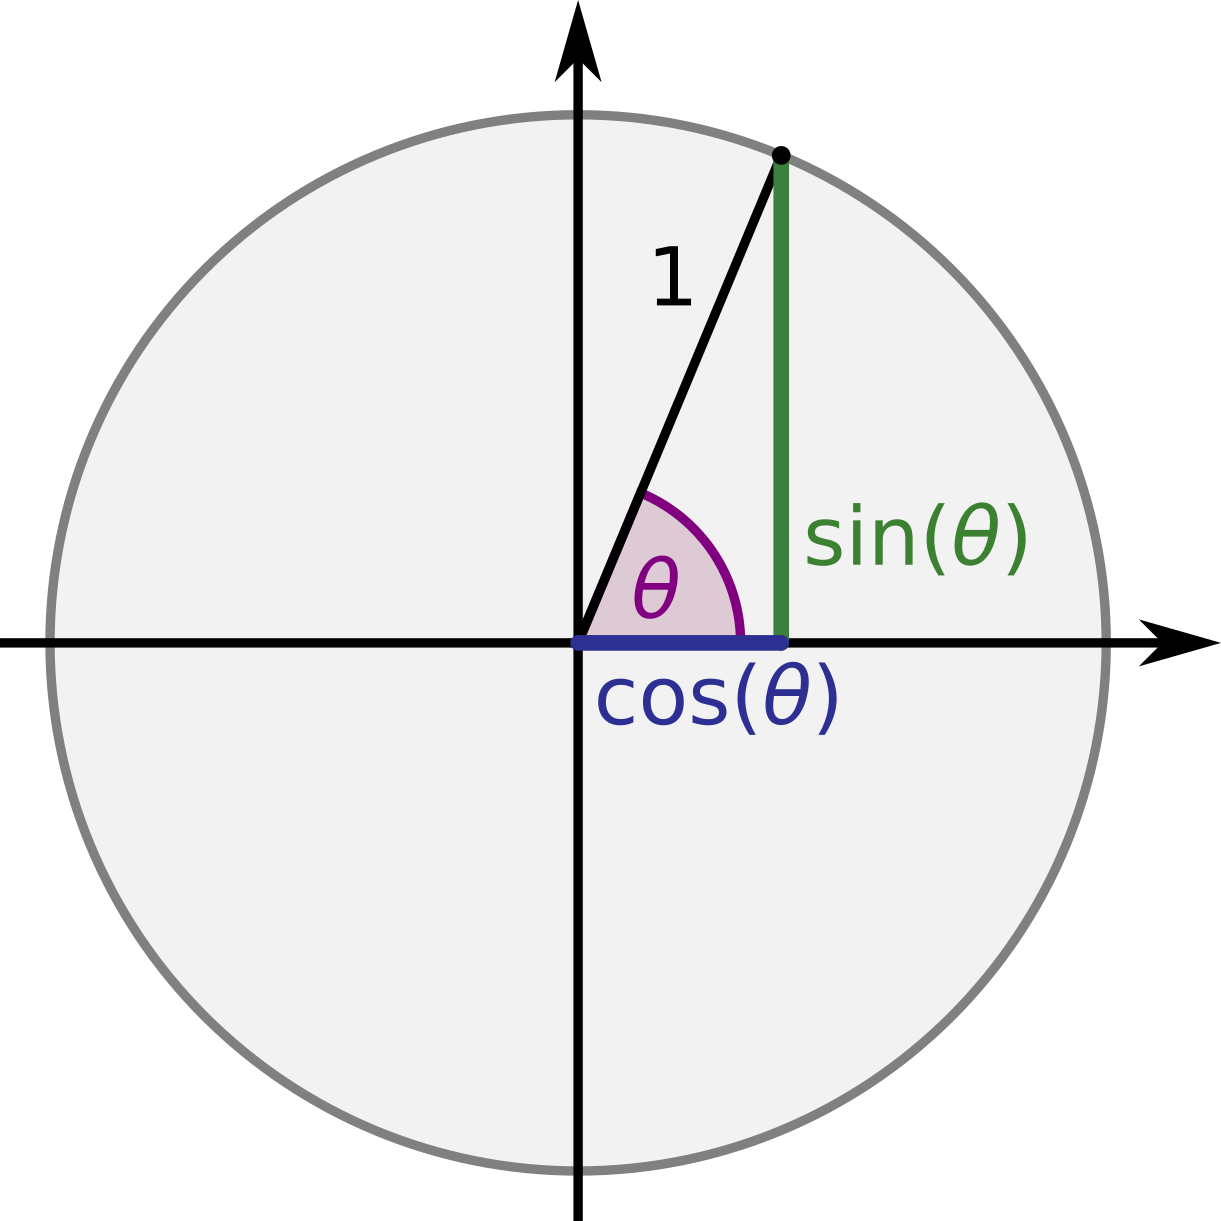
\includegraphics[width=0.5\textwidth]{Einheitskreis.png}
\end{center}



\end{frame}




%% Review



\begin{frame}

\frametitle{Jetzt* sollten Sie:}



\begin{block}{Wissen:}
\begin{itemize}
\item
Basiseinheiten und häufige abgeleitete Einheiten des SI-Systems benennen
\item
Messunsicherheit erklären
\item
 Vektoren, Skalare, Exponentialfunktionen, Logarithmen, Trigonometrischen Funktionen, Integration und Differentialrechnung erklären
\item 
Mittelwert, Standardabweichung, und Standardabweichung des Mittelwerts erklären 
\item
Eigenschaften der Gaußschen Glockenkurve benennen
\end{itemize}
\end{block}

\end{frame}

\begin{frame}

\frametitle{Jetzt* sollten Sie:}
 



\begin{block}{Können:}
\begin{itemize}
\item
 dezimale Vielfache von Einheiten sprachlich und durch Zehnerpotenzen darstellen
\item
 mit Messgrößen rechnen
\item
 Messunsicherheit darstellen und abschätzen
\item
 Mittelwert, Standardabweichung, und Standardabweichung des Mittelwerts berechnen
\item 
mit Funktionsgraphen arbeiten
\end{itemize}
\end{block}

 
\begin{block}{Fühlen:}
\begin{itemize}
\item
erkennen, warum Physik in der Medizin wichtig ist
\item
verstehen, warum manche Konzepte (Gaußsche Glockenkurve, Logarithmen, Differential etc.) oft vorkommen
\item
 rechnen ohne Angst
\end{itemize}
\end{block}

\end{frame}


%% Feedbackhinweisblock
\begin{frame}
\frametitle{Danke für Ihr Feedback!}

\begin{columns}[c]

\begin{column}{6cm}
\begin{center}
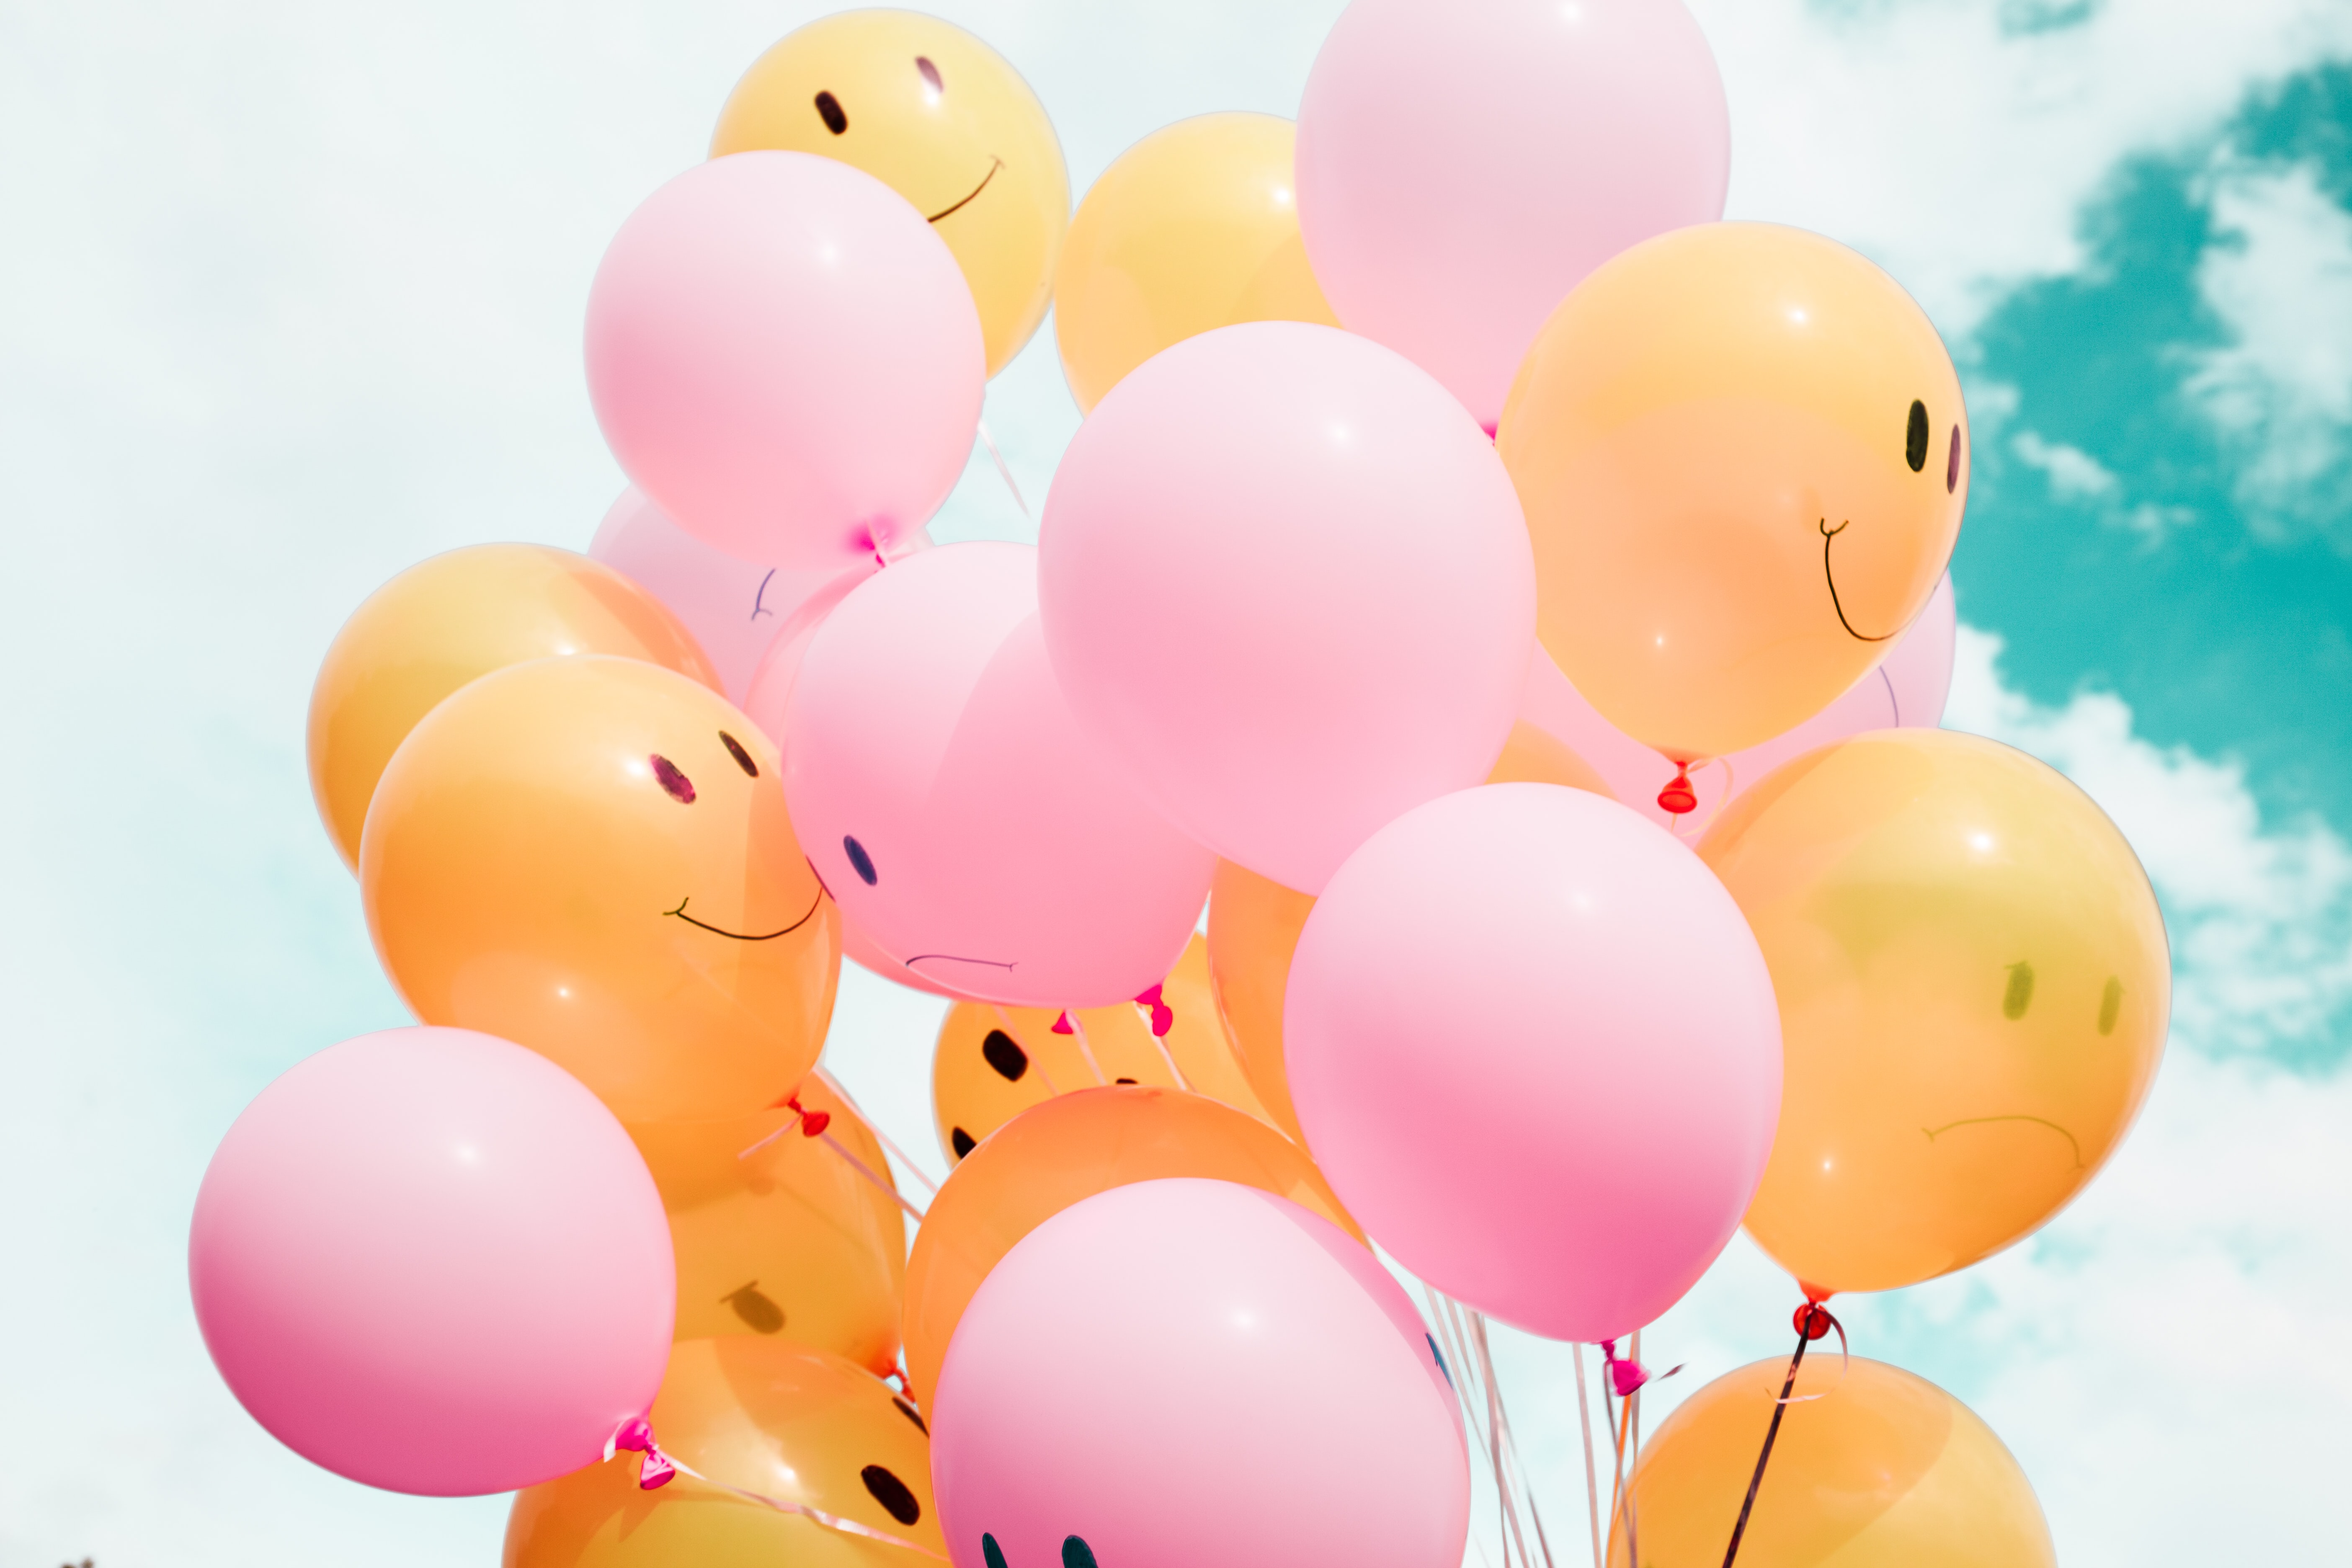
\includegraphics[width=\textwidth]{smilie_balloons.jpg}
\end{center}

\end{column}

\begin{column}{4cm}


\begin{center}

\includegraphics[width=\textwidth]{feedback_QR.png}
\end{center}
\end{column}


\end{columns}

\end{frame}




%% Bildnachweis
\begin{frame}
\frametitle{Bildnachweis}

Diese Vorlesung verwendet teilweise Materialien (Folien und Bilder) einer früheren Vorlesung von Prof. Wim Walter.  

\vfill

\begin{tiny}
 
\begin{itemize}

\item
\item
Ausgestreckte Hand mit Apfel. Photo by \href{https://unsplash.com/@priscilladupreez?utm_source=unsplash&utm_medium=referral&utm_content=creditCopyText}{Priscilla Du Preez} on \href{https://unsplash.com/s/photos/apple?utm_source=unsplash&utm_medium=referral&utm_content=creditCopyText}{Unsplash}


\item
 68 - 95 - 99.7 Regel. By M. W. Toews - Own work, based (in concept) on figure by Jeremy Kemp, on 2005-02-09, CC BY 2.5, \url{https://commons.wikimedia.org/w/index.php?curid=1903871}, via Wikimedia Commons


\item
Coronavirus. By NIAID - \url{https://www.flickr.com/photos/niaid/49534865371/}, CC BY 2.0, \url{https://commons.wikimedia.org/w/index.php?curid=92612457}
\item
Covid-19 Infektionen in Afrika. Aus: Musa, S.S., Zhao, S., Wang, M.H. et al. Estimation of exponential growth rate and basic reproduction number of the coronavirus disease 2019 (COVID-19) in Africa. Infect Dis Poverty 9, 96 (2020). \url{https://doi.org/10.1186/s40249-020-00718-y}



\item
Einheitskreis. By Stephan Kulla (User:Stephan Kulla) - Own work, CC0, \url{https://commons.wikimedia.org/w/index.php?curid=57551646}

\item
Ergebnisse beim Würfeln. Meine eigene Arbeit, CC-BY-SA 4.0, 2021.

\item

Formeln und Diagramme mit Giraffen. Eigene Arbeit, 2022. CC-BY-SA 4.0.

\item 
Frau mit großem Einkaufskorb. Photo by \href{https://unsplash.com/@ibilyk?utm_source=unsplash&utm_medium=referral&utm_content=creditCopyText}{Liuba Bilyk} on \href{https://unsplash.com/s/photos/carrying-groceries?utm_source=unsplash&utm_medium=referral&utm_content=creditCopyText}{Unsplash}


\item
Frustrierter und verwirrter Mensch. Photo by \href{https://unsplash.com/@officestock?utm_source=unsplash&utm_medium=referral&utm_content=creditCopyText}{Sebastian Herrmann} on \href{https://unsplash.com/s/photos/frustration?utm_source=unsplash&utm_medium=referral&utm_content=creditCopyText}{Unsplash}

\item
Funktionsgraphen mit Differential und Integral. Meine eigene Arbeit, CC-BY-SA 4.0.


\item
Giraffen unterschiedlicher Größe. Photo by \href{https://unsplash.com/@perventuator?utm_source=unsplash&utm_medium=referral&utm_content=creditCopyText}{Bibhash (Knapsnack.life) Banerjee} on \href{https://unsplash.com/s/photos/giraffe?utm_source=unsplash&utm_medium=referral&utm_content=creditCopyText}{Unsplash}
  


\item
Graphen von Körpergewicht und 5-Kilometer Zeit. Eigene Arbeit, 2022. CC-BY-SA 4.0.
  \item
Lauf-Event. Photo by \href{https://unsplash.com/@capstoneeventgroup?utm_source=unsplash&utm_medium=referral&utm_content=creditCopyText}{Capstone Events} on \href{https://unsplash.com/s/photos/marathon?utm_source=unsplash&utm_medium=referral&utm_content=creditCopyText}{Unsplash}
\item
Logo der MSB. MSB Medical School Berlin, Public Domain, via Wikimedia Commons

\item
Luftballons mit frohen und traurigen Smileys. Photo by \href{https://unsplash.com/@artbyhybrid?utm_source=unsplash&utm_medium=referral&utm_content=creditCopyText}{Hybrid} on \href{https://unsplash.com/s/photos/feedback?utm_source=unsplash&utm_medium=referral&utm_content=creditCopyText}{Unsplash}


\item
Screenshot eines Artikels über einen Asteroiden-Einschlag. Daily Mail Online vom 14.3.2022.
\item
Studentin präsentiert Daten. Von Yuuki Guzman und Agoston Tyll, Okinawa Institute of Science and Technology, 2015, mit Erlaubnis. 
\item
Übersicht Modul Physik. Meine eigene Arbeit, CC-BY-SA 4.0, 2023. 
\item
Vektoren. Meine eigene Arbeit, CC-BY-SA 4.0, 2022.
\end{itemize}

\end{tiny}
\end{frame}












\end{document}




